\section{Requisitos da Experiência Meta 4}
Para este estudo experimental foi criado um cluster Multi-Master com recurso ao MariaDB e Galera.

Virtualizador: VMware Workstation Pro 16.2.0 (Licensed)

Sistema Operativo: Linux Ubuntu 22.04:
\url{https://ubuntu.com/download/desktop}

MariaDB: 10.6.7

Mysql: 15.1

Galera: 4

\begin{figure}[H]
\center
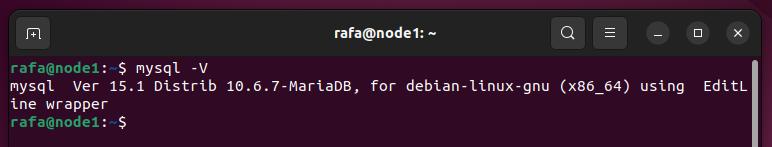
\includegraphics[width=12cm]{version.png}
\caption{Versão}
\end{figure}

\indent Endereçamento:
\begin{table}[h]
\begin{center}
\begin{tabular}{||c c||} 
 \hline
 Nome & IP\\ [0.5ex] 
 \hline\hline
 Node 1 & 192.168.1.118\\ 
 \hline
 Node 2 & 192.168.1.119\\
 \hline
 Node 3 & 192.168.1.120\\
 \hline
 Sysbench & 192.168.1.121\\
 \hline
 Proxy & 192.168.1.122\\
 \hline
\end{tabular}
\caption{Tabela endereçamento IP Meta 4}
\end{center}
\end{table}

\newpage
\section{Instalação Ubuntu}

Nesta secção explico passo a passo a instalação da \ac{VM} Ubuntu, nó 1. A instalação das outras \ac{VM} é repetir o mesmo processo.


Passo 1: "Create a new virtual machine".
\begin{figure}[H]
\center
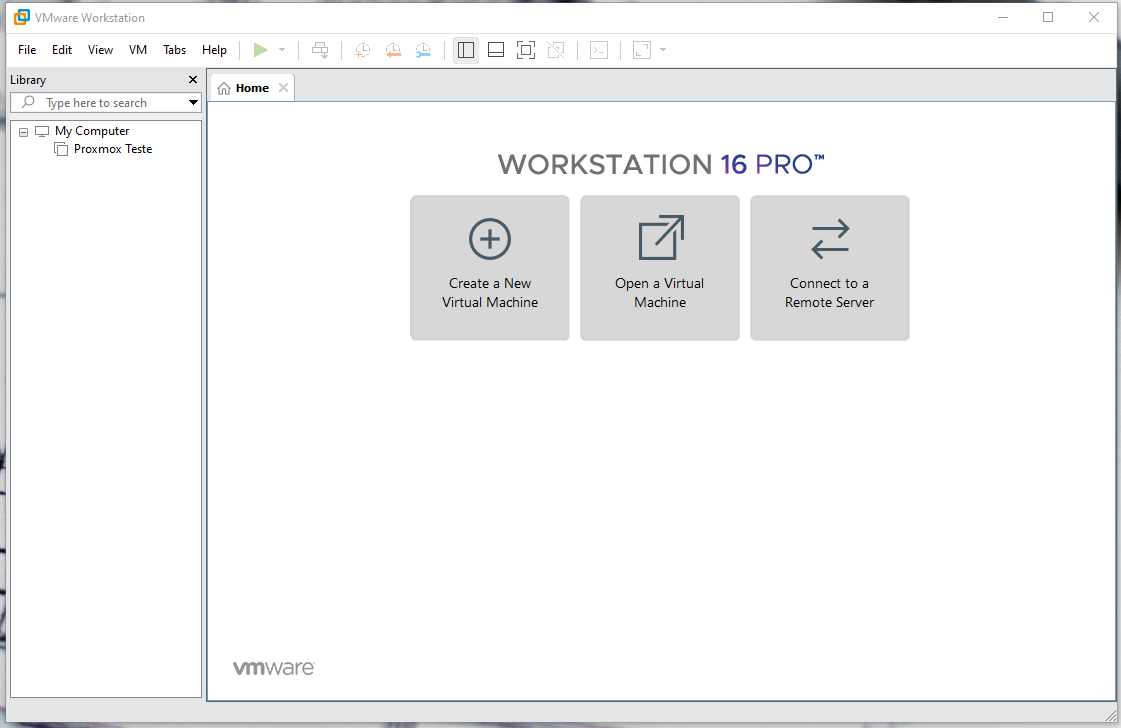
\includegraphics[width=13cm]{1.png}
\caption{Create a new virtual machine}
\end{figure}

Passo 2: Aqui é escolha pessoal, eu escolhi a "Typical".
\begin{figure}[H]
\center
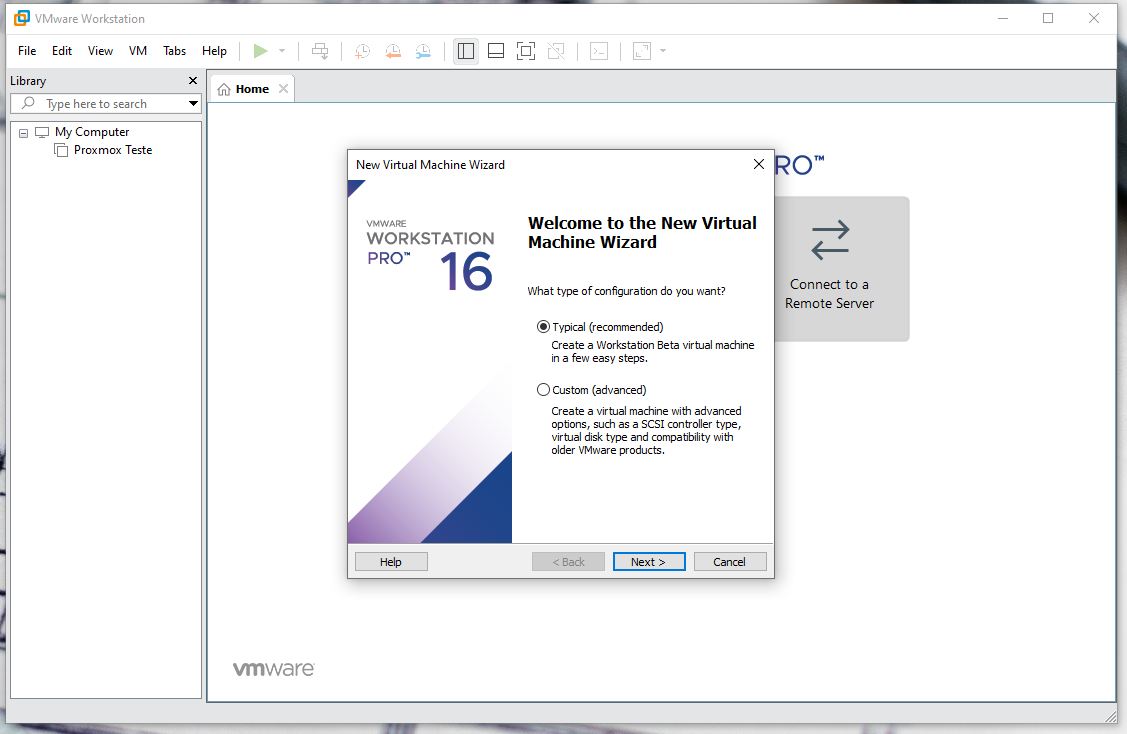
\includegraphics[width=13cm]{2.png}
\caption{Tipo de configuração}
\end{figure}

\newpage
Passo 3: Escolher instalar o Sistema Operativo mais tarde.
\begin{figure}[H]
\center
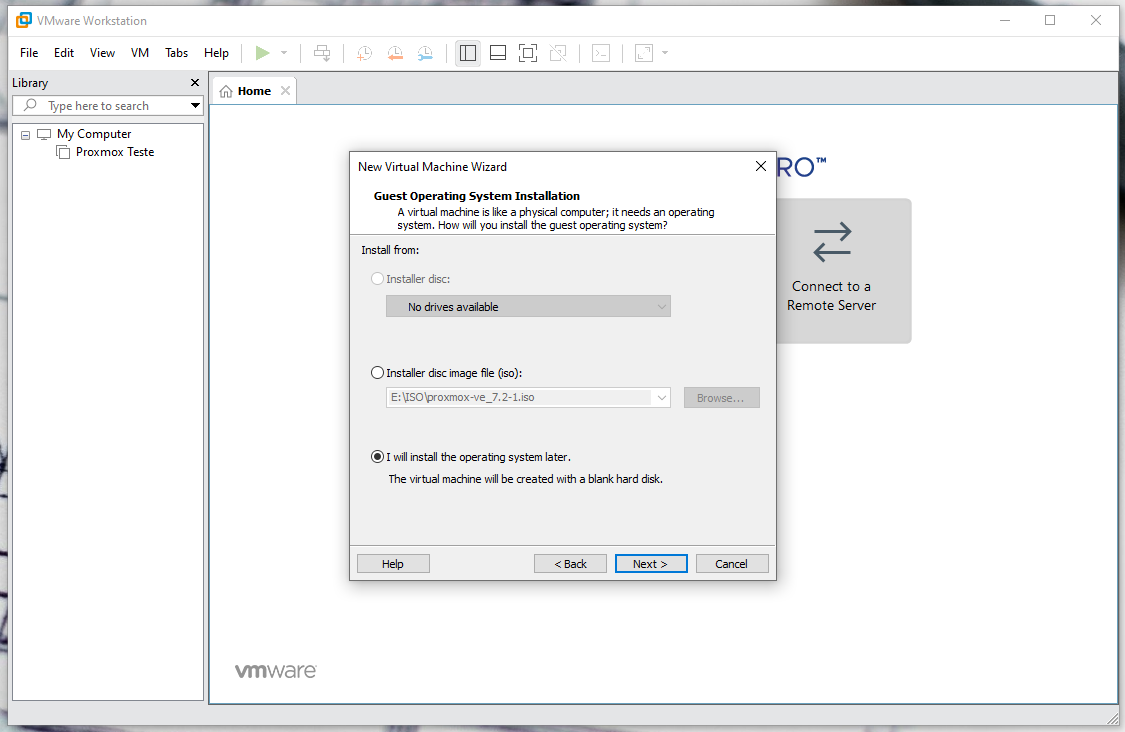
\includegraphics[width=13cm]{3.png}
\caption{Install the Operatin System later}
\end{figure}

Passo 4: Por pré-definição deixei ficar as opções dadas uma vez que também ia instalar Ubuntu.
\begin{figure}[H]
\center
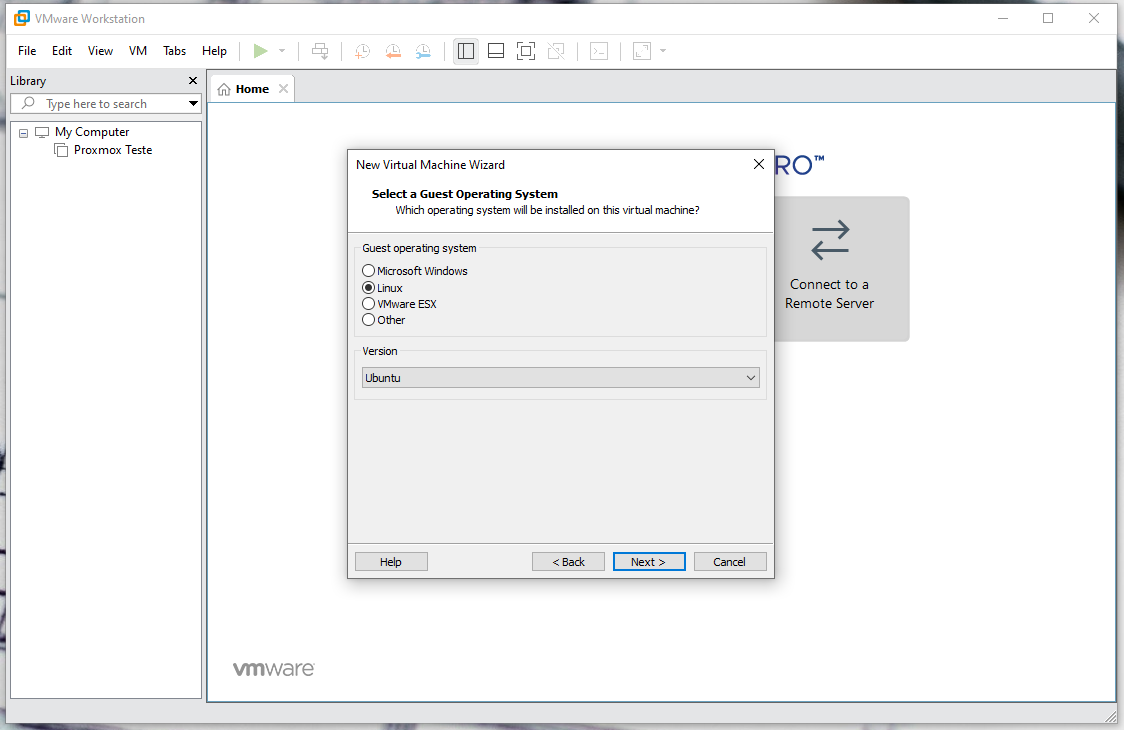
\includegraphics[width=13cm]{4.png}
\caption{Tipo Sistema Operativo}
\end{figure}

\newpage
Passo 5: Escolher o nome para a \ac{VM} e a localização.
\begin{figure}[H]
\center
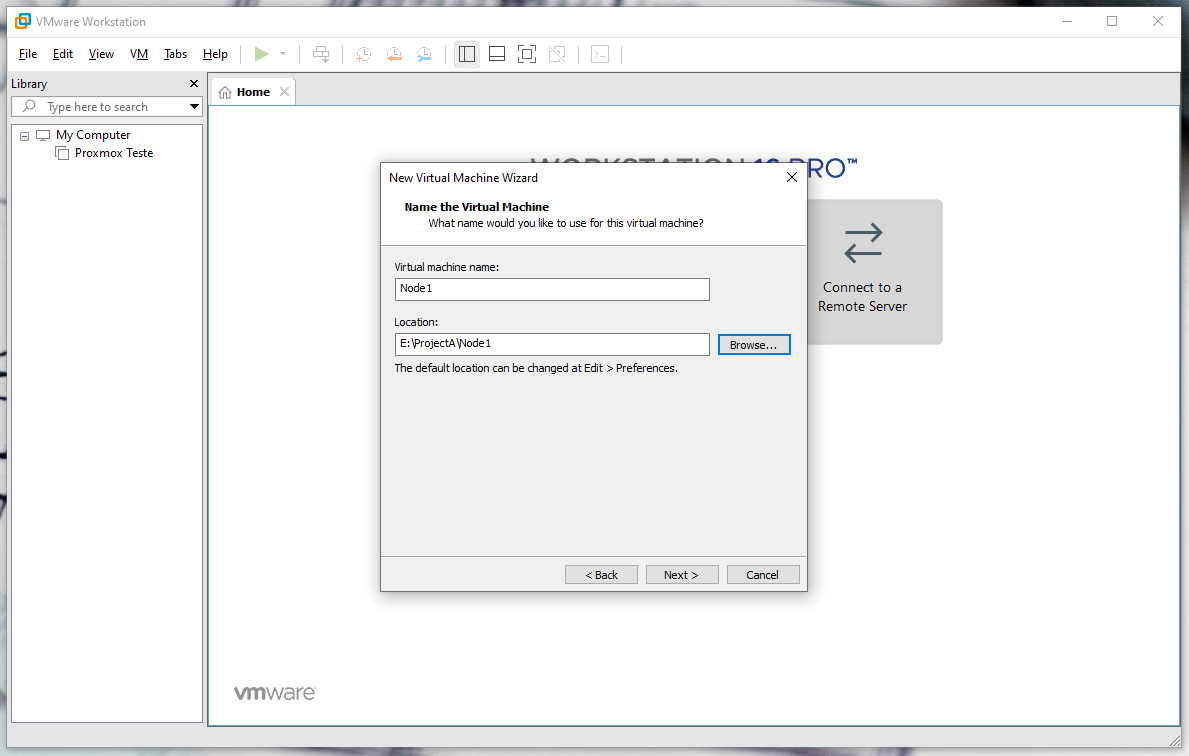
\includegraphics[width=13cm]{5.png}
\caption{Nome e localização da \ac{VM}}
\end{figure}

Passo 6: Definir tamanho do disco para a \ac{VM}.
\begin{figure}[H]
\center
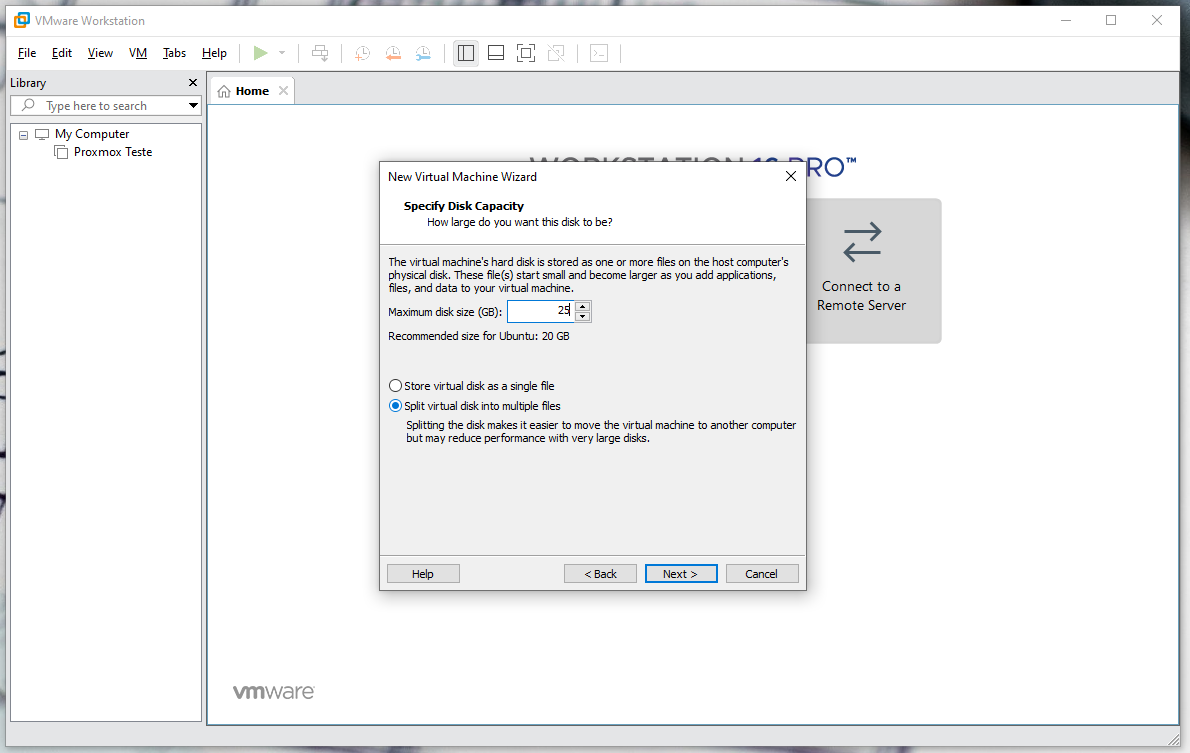
\includegraphics[width=13cm]{6.png}
\caption{Tamanho Disco \ac{VM}}
\end{figure}

\newpage
Passo 7: Resumo da configuração e finalização.
\begin{figure}[H]
\center
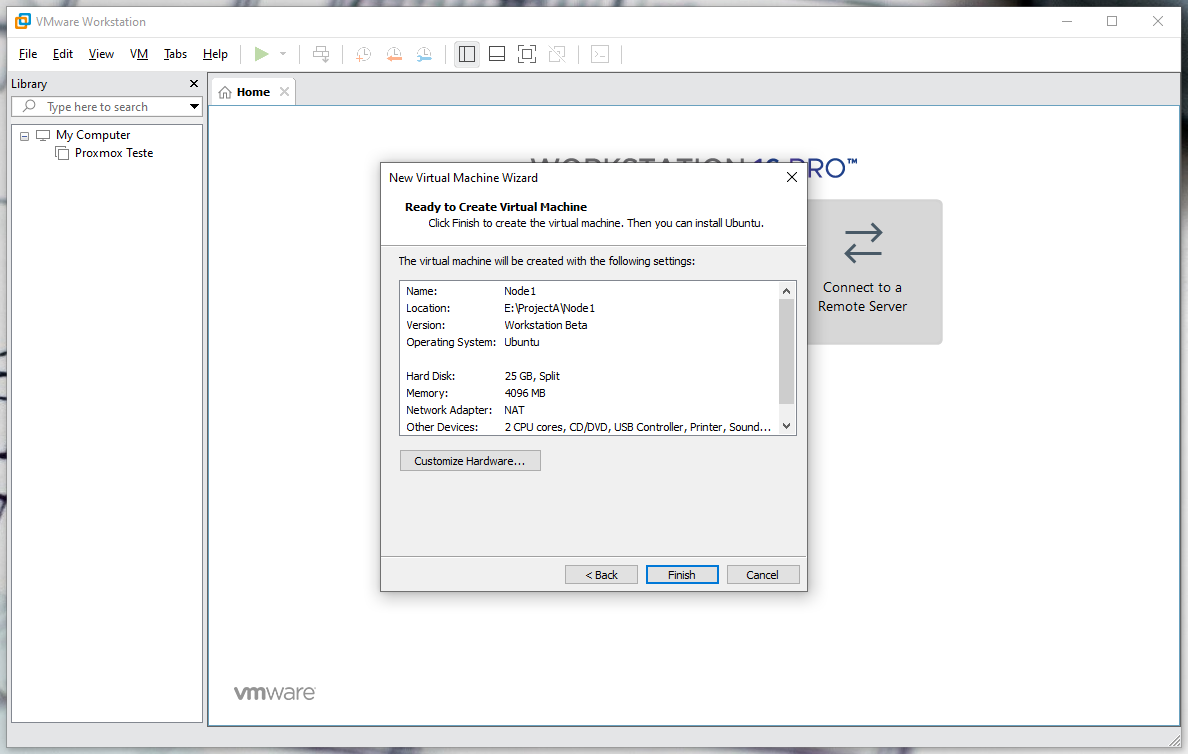
\includegraphics[width=13cm]{7.png}
\caption{Finalização}
\end{figure}

Passo 8: Neste passo vamos ás propriedades da \ac{VM} inserir a \ac{ISO} do Ubuntu em "\ac{CD/DVD} (\ac{SATA})".
\begin{figure}[H]
\center
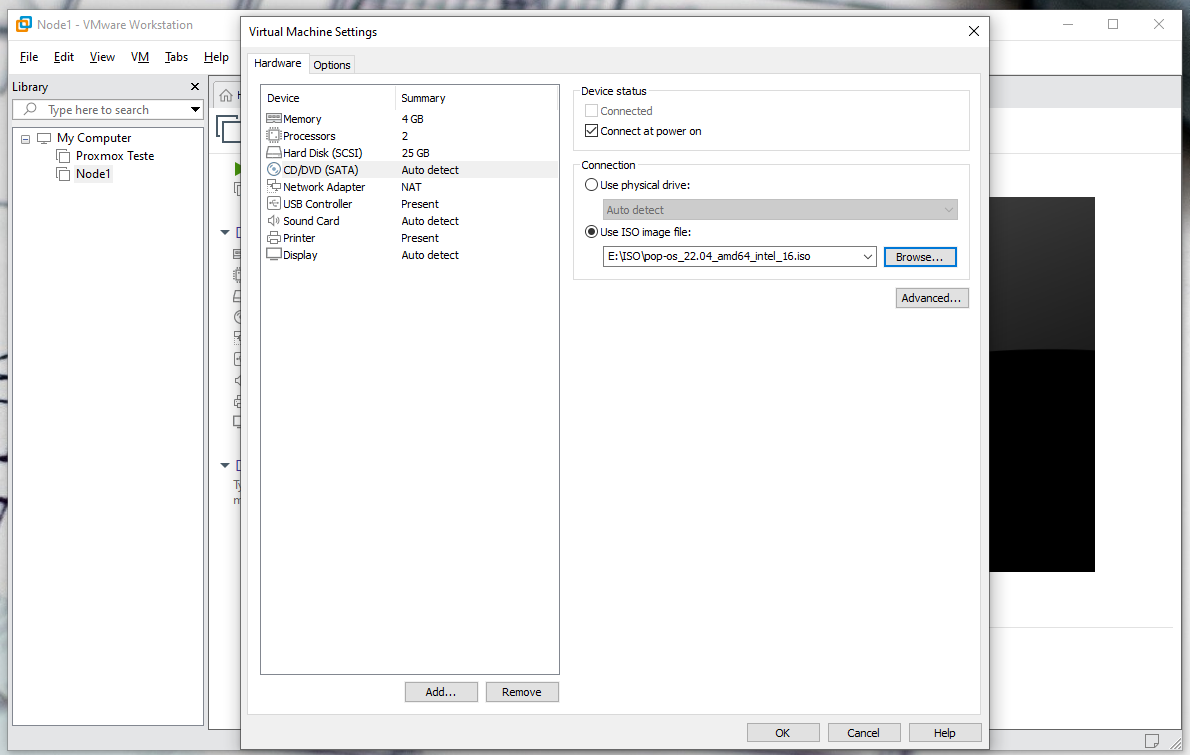
\includegraphics[width=13cm]{8.png}
\caption{Inserir \ac{ISO}}
\end{figure}


\newpage
Passo 9: Depois de definir a \ac{ISO} no passo anterior, é hora de dar "START" a \ac{VM} para iniciar as instalação do Ubuntu.
\begin{figure}[H]
\center
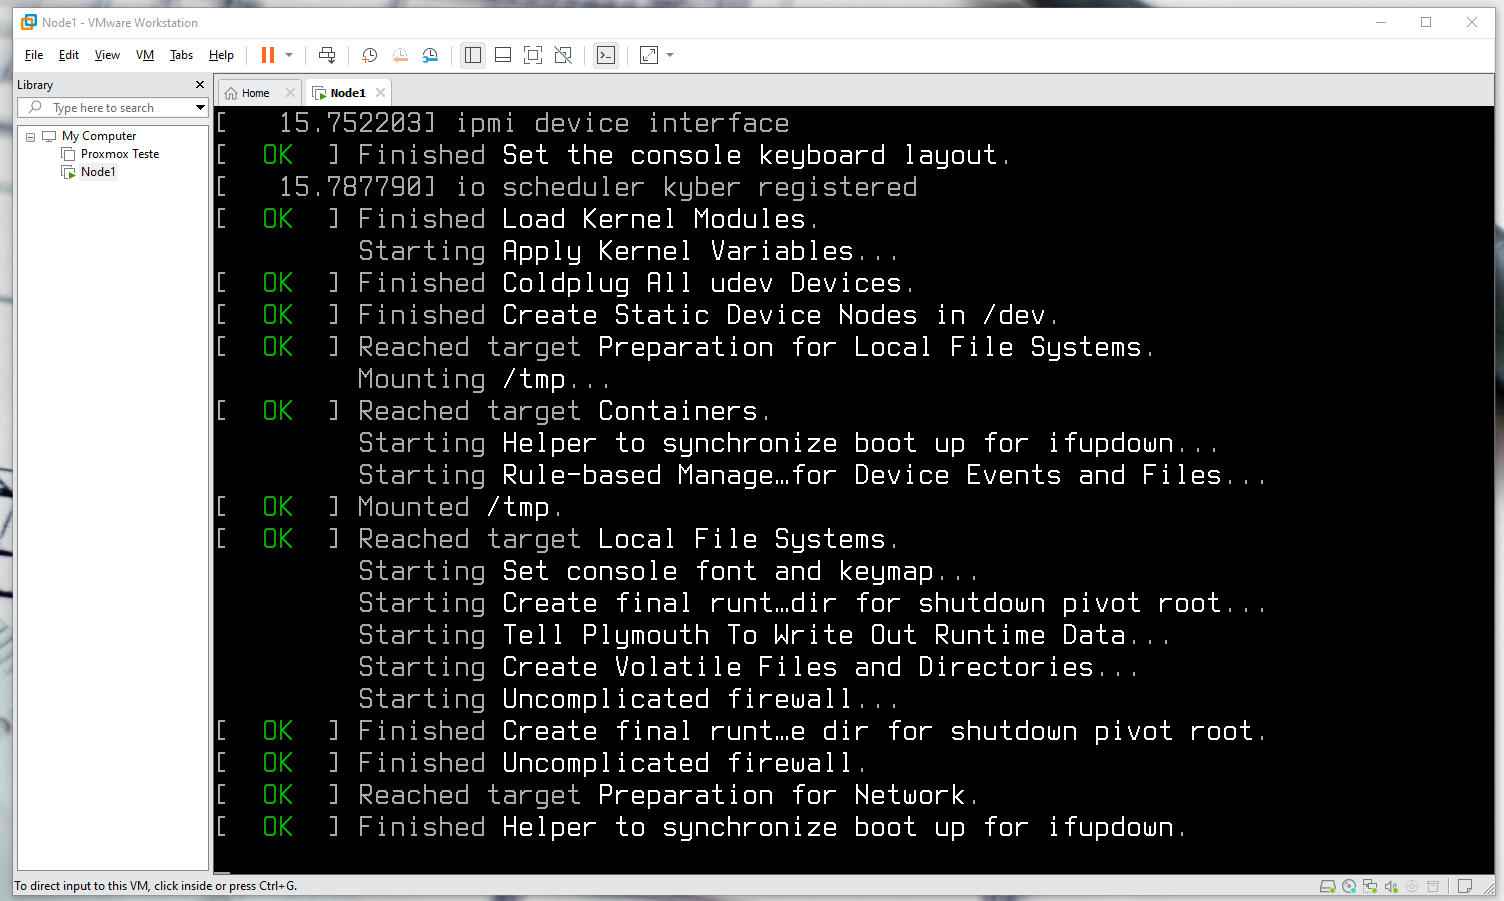
\includegraphics[width=13cm]{9.png}
\caption{Inicialização VM}
\end{figure}

Passo 10: "Instalar o Ubuntu".
\begin{figure}[H]
\center
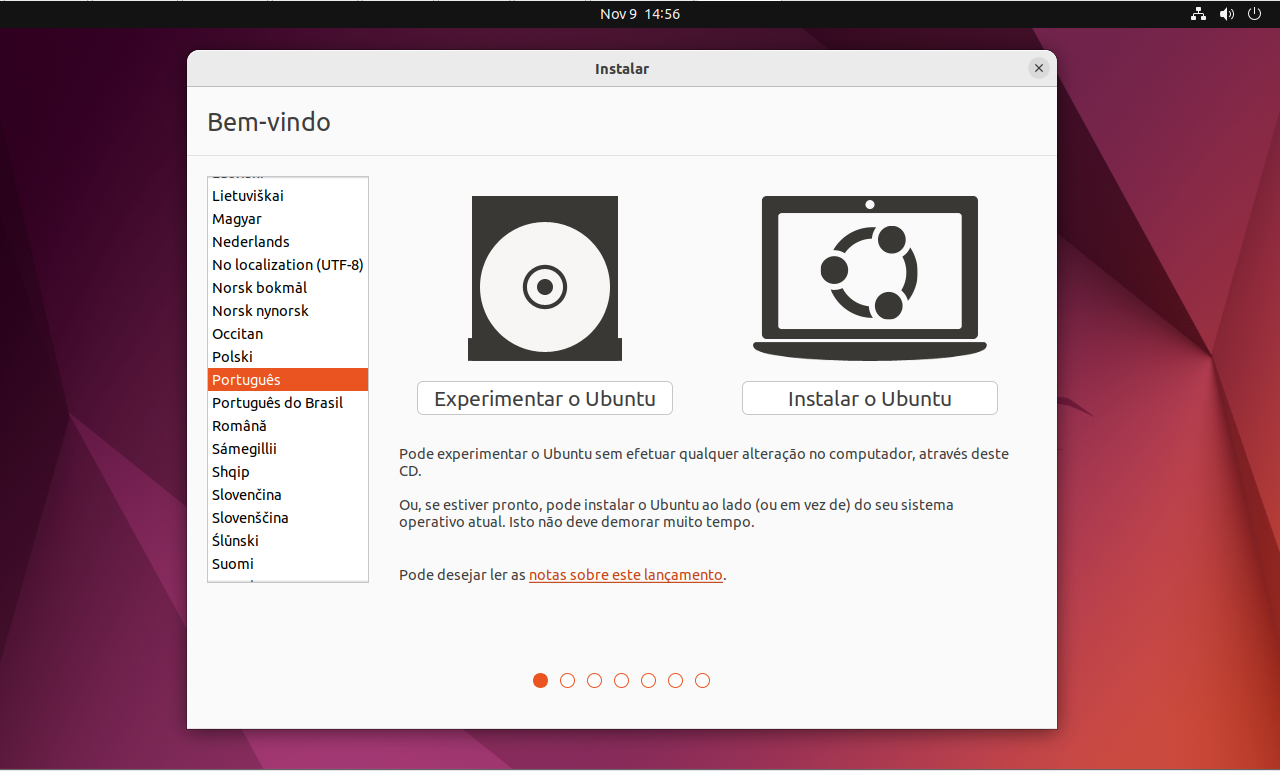
\includegraphics[width=13cm]{10.png}
\caption{Instalar Ubuntu}
\end{figure}

\newpage
Passo 11: Idioma teclado.
\begin{figure}[H]
\center
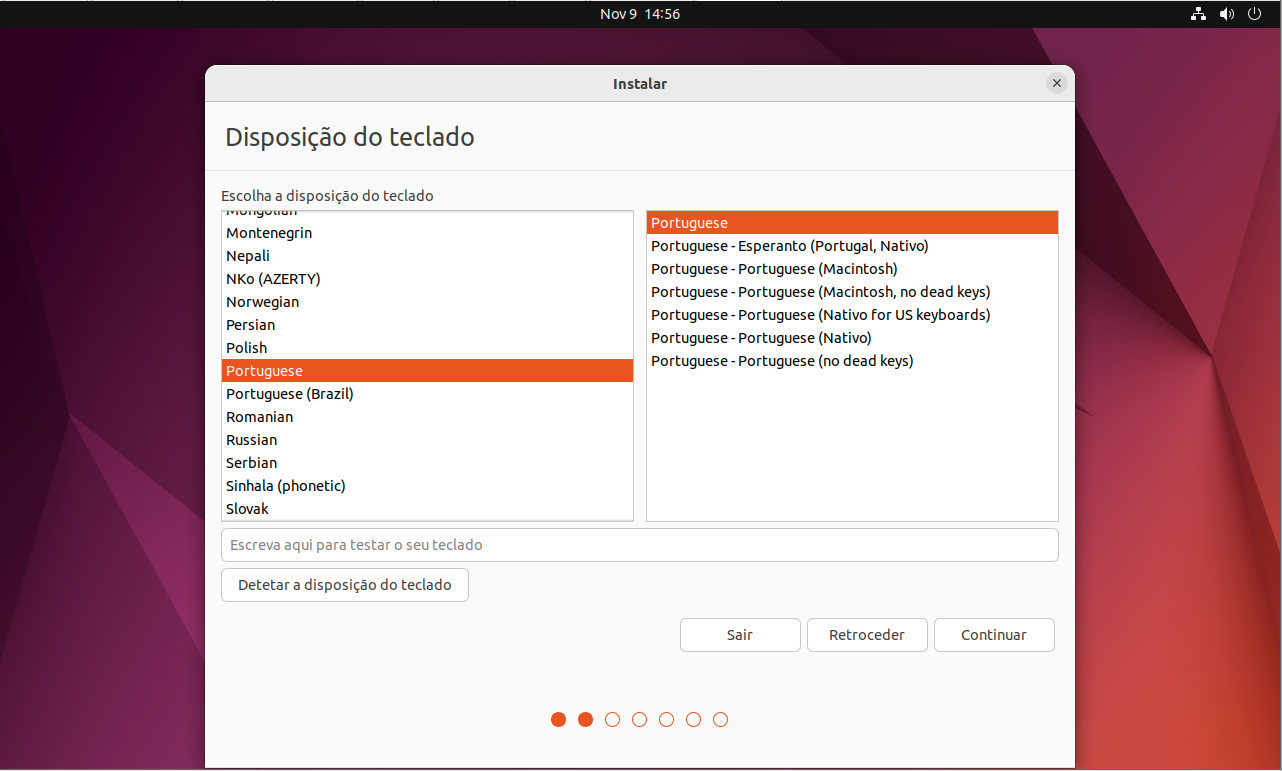
\includegraphics[width=13cm]{11.png}
\caption{Idioma teclado}
\end{figure}

Passo 12: Atualizações (por defeito não alterei nada).
\begin{figure}[H]
\center
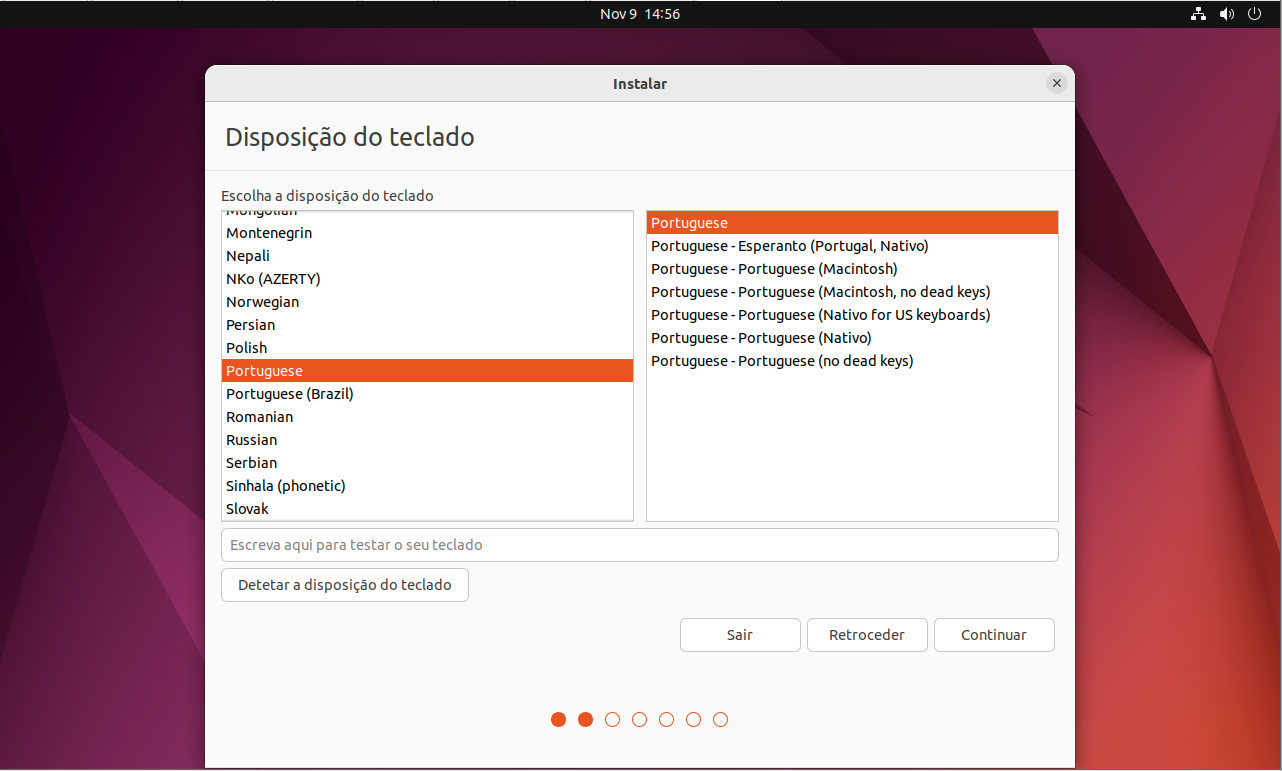
\includegraphics[width=13cm]{11.png}
\caption{Atualizações}
\end{figure}

\newpage
Passo 13: Escolher o tipo de instalação (optei por "Apagar disco e instalar o Ubuntu".
\begin{figure}[H]
\center
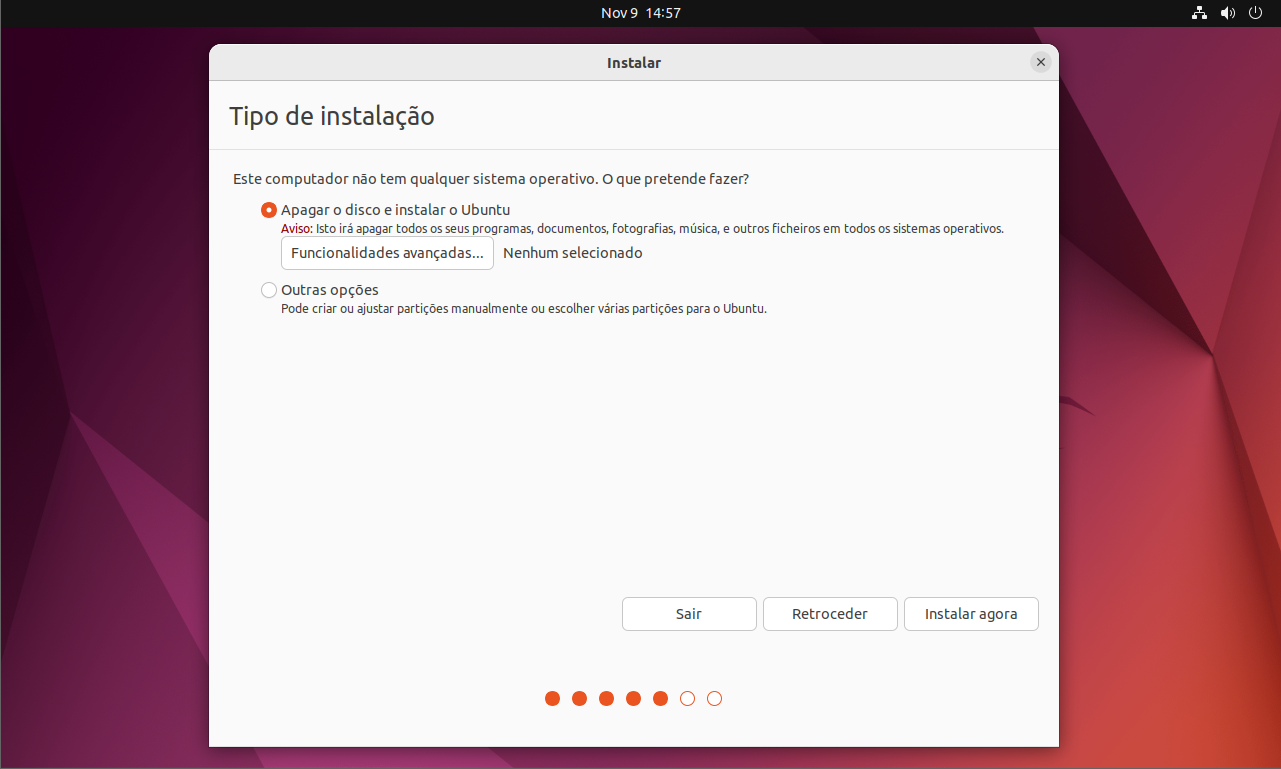
\includegraphics[width=13cm]{13.png}
\caption{Tipo de instalação}
\end{figure}

Passo 14: Conformação das alterações dos discos, "Continuar".
\begin{figure}[H]
\center
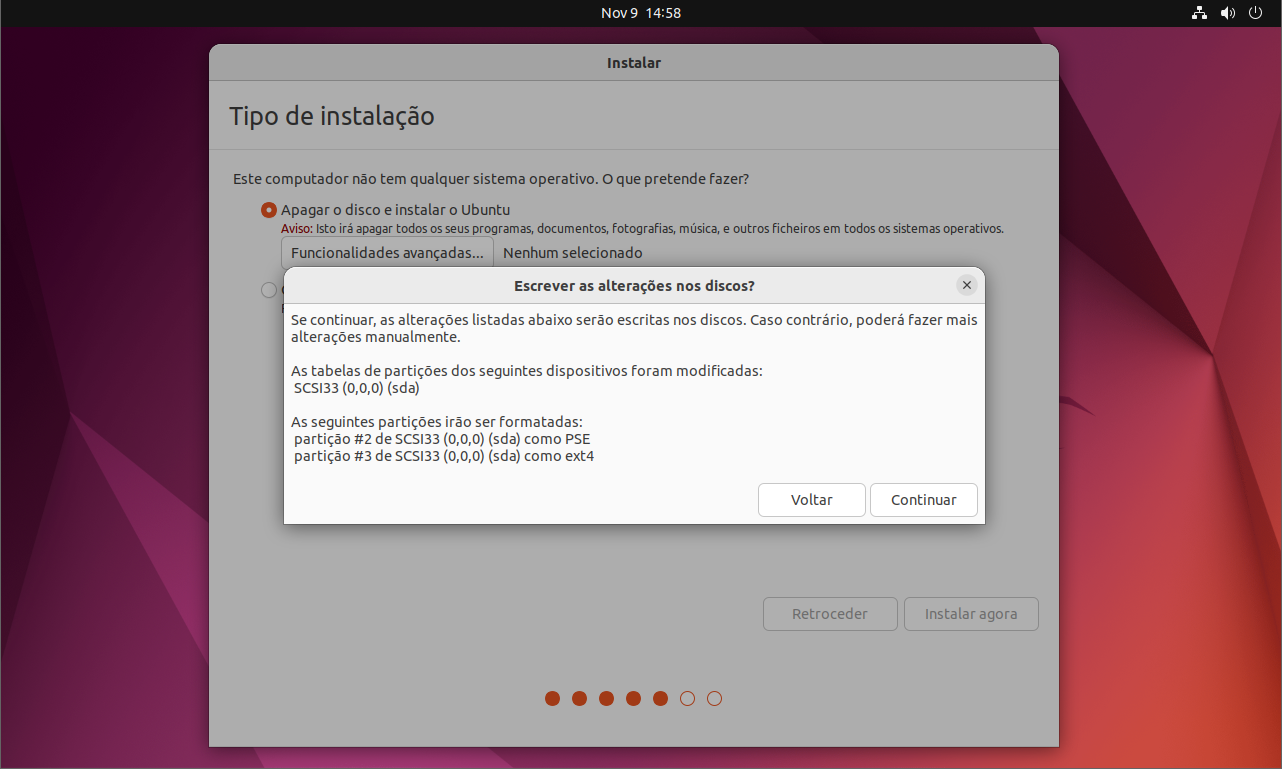
\includegraphics[width=13cm]{14.png}
\caption{Confrmação}
\end{figure}

\newpage
Passo 15: Escolha da localização.
\begin{figure}[H]
\center
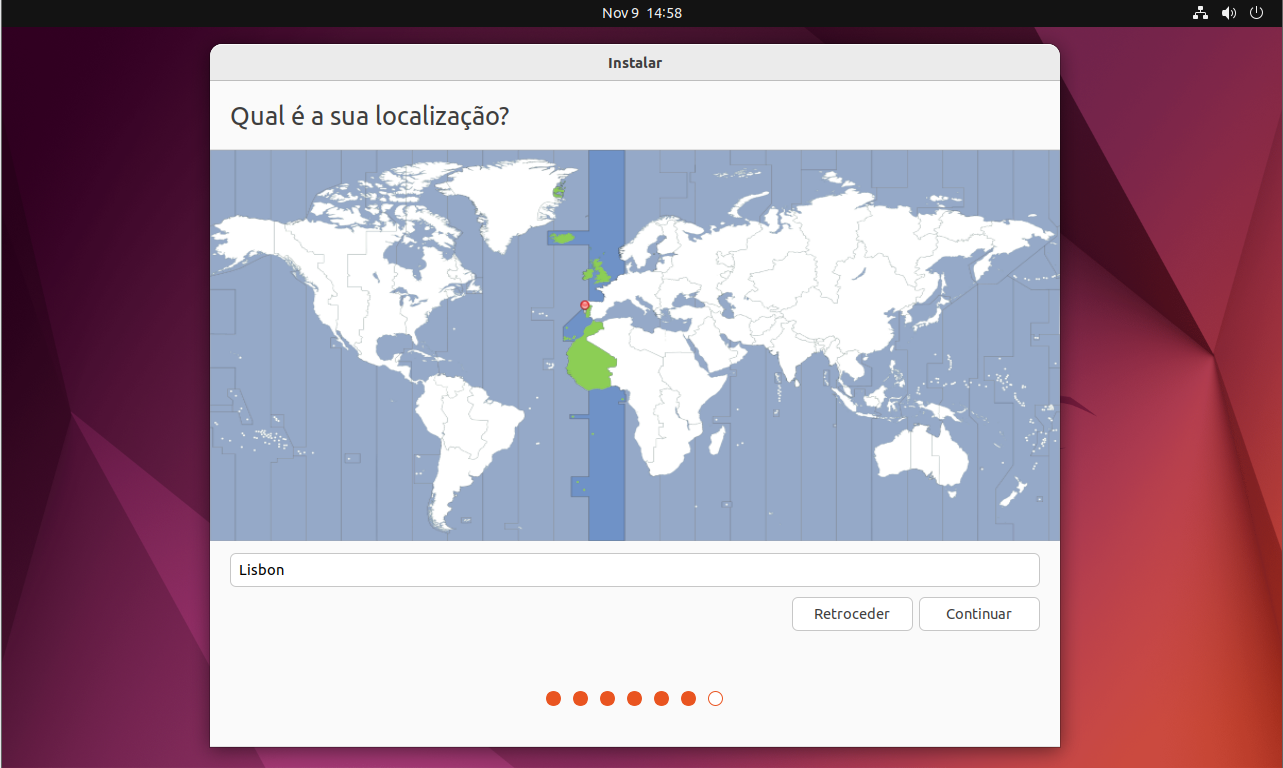
\includegraphics[width=13cm]{15.png}
\caption{Localização}
\end{figure}

Passo 16: Processo de definir o nome, o nome da maquina, o nome de utilizador e password.
\begin{figure}[H]
\center
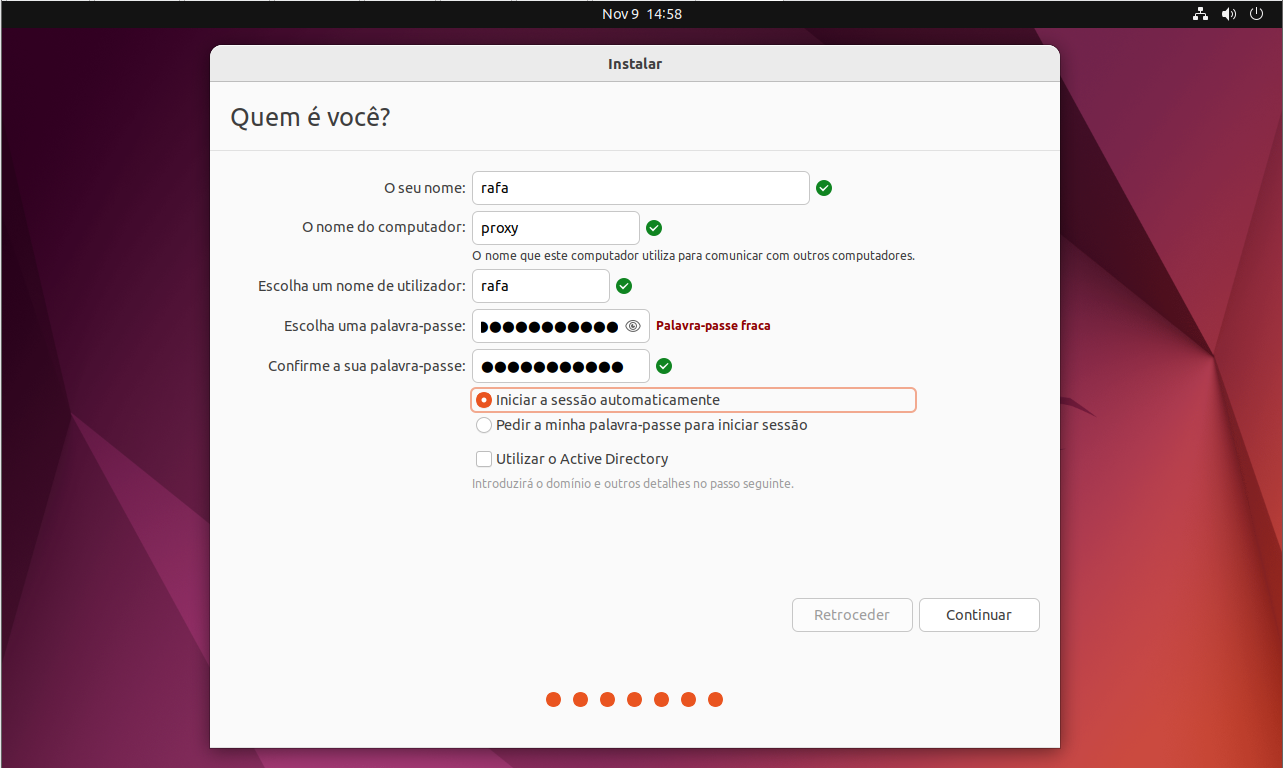
\includegraphics[width=13cm]{16.png}
\caption{Informações pessoais}
\end{figure}

\newpage
Passo 17: Instalação do Ubuntu.
\begin{figure}[H]
\center
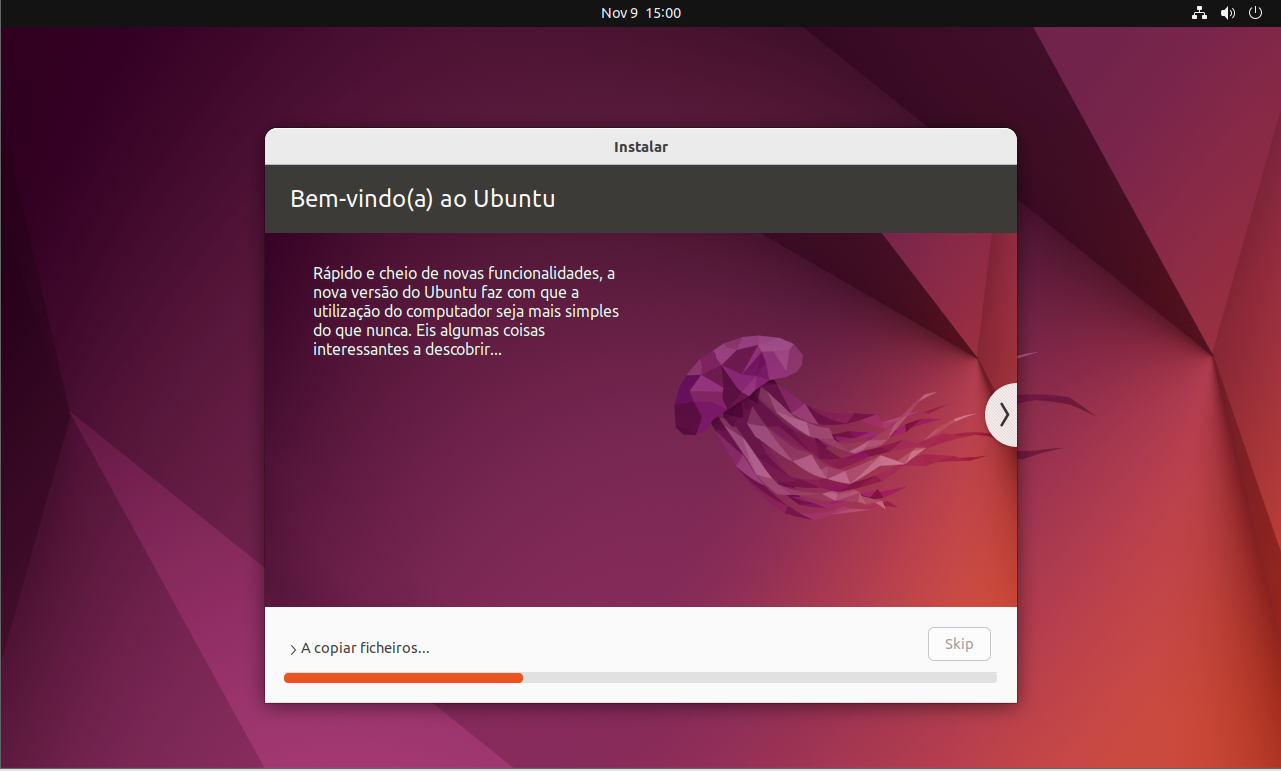
\includegraphics[width=13cm]{17.png}
\caption{Instalação}
\end{figure}

Passo 18: Finalizada a instalação apenas basta reiniciar e entrar no \ac{SO}.
\begin{figure}[H]
\center
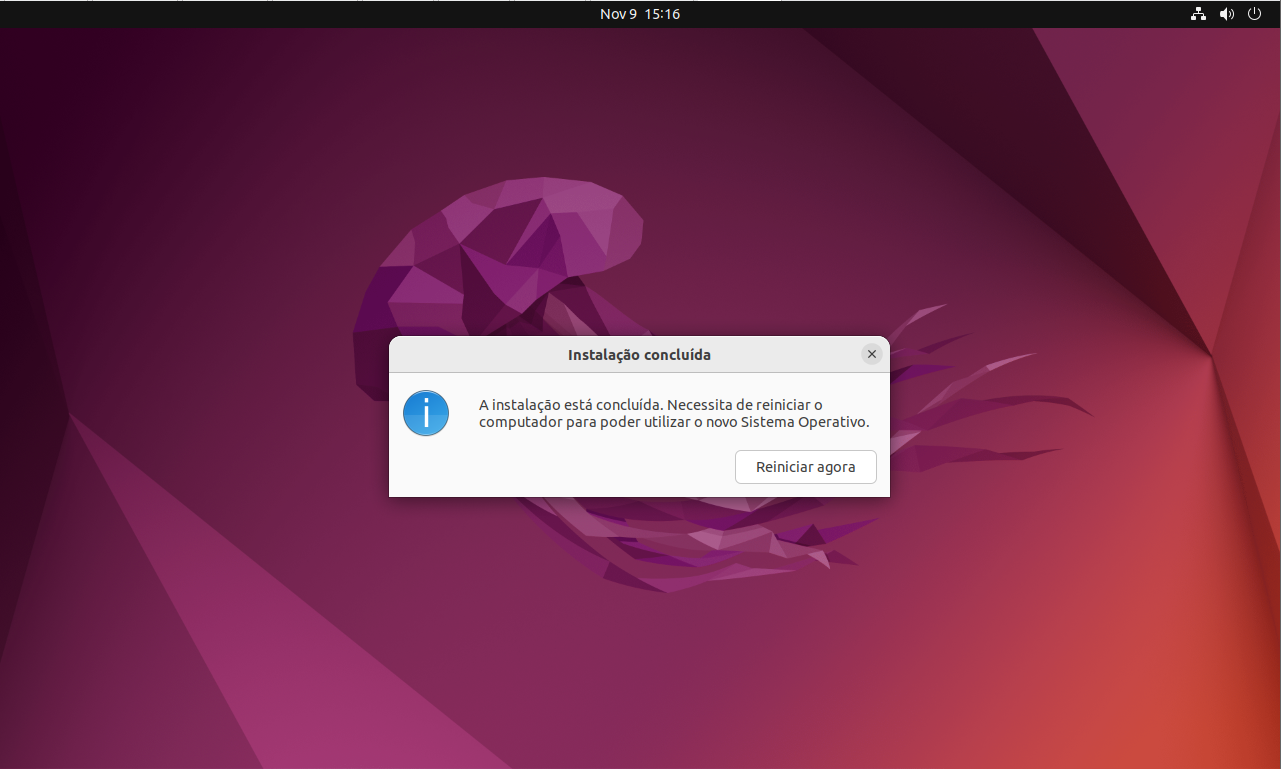
\includegraphics[width=13cm]{18.png}
\caption{Riniciar o Sistema Operativo}
\end{figure}

NOTA: nas propriedades da \ac{VM}, em \ac{CD/DVD} (\ac{SATA}), desmarquei a opção de "Use ISO file" para "Use physical drive", para a \ac{VM} não arrancar através da \ac{ISO} e sim pelo sistema instalado no disco.

\newpage
\section{Portas Firewall}
Numa primeira fase do projeto fui verificando os vários processos para a implementação desta Meta 4 e percebi que iria precisar de implementar regras para a firewall das \ac{VM} para os vários serviços. E por isso inicialmente começo por adicionar algumas das portas necessárias:

\subsection{Portas usadas:}
\begin{itemize}
    \item 3306: Serviço MySQL;
    \item 4567: Tráfego de Replicação do Galera Cluster;
    \item 4568: \ac{IST};
    \item 4444: \ac{SST};
    \item 80: \ac{HTTP};
    \item 22: \ac{SSH};    
\end{itemize}

\hfill \break
Podia adicionar ao arquivo \textit{/etc/sysconfig/iptables} a configuração das \textit{iptables}, mas optei por configurar no terminal da \ac{VM}:
\begin{verbatim} sudo ufw enable \end{verbatim}
\begin{verbatim} sudo ufw allow 3306,4567,4568,4444,80,22,6033/tcp \end{verbatim}
\begin{verbatim} sudo ufw allow 4567/udp \end{verbatim}
\begin{verbatim} sudo ufw reload \end{verbatim}

\newpage
\section{Instalação MariaDB + Galera}

NOTA IMPORTANTE: Todos os passos seguintes devem ser replicados pelas restantes \ac{VM}, Node2 e Node3.

Para este estudo experimental optei por instalar o MariaDB uma vez que nas versões recentes já inclui o galera.
Para começar, atualiza-se os repositórios locais do Ubuntu através do terminal:

\begin{verbatim} sudo apt update \end{verbatim}

De seguida instalei o MariaDB server:
\begin{verbatim} sudo apt install mariadb-server \end{verbatim}

Depois de concluída a instalação do MariaDB server podemos verificar qual as versões instaladas:

\begin{verbatim} mariadb --version \end{verbatim}

\begin{figure}[H]
\center
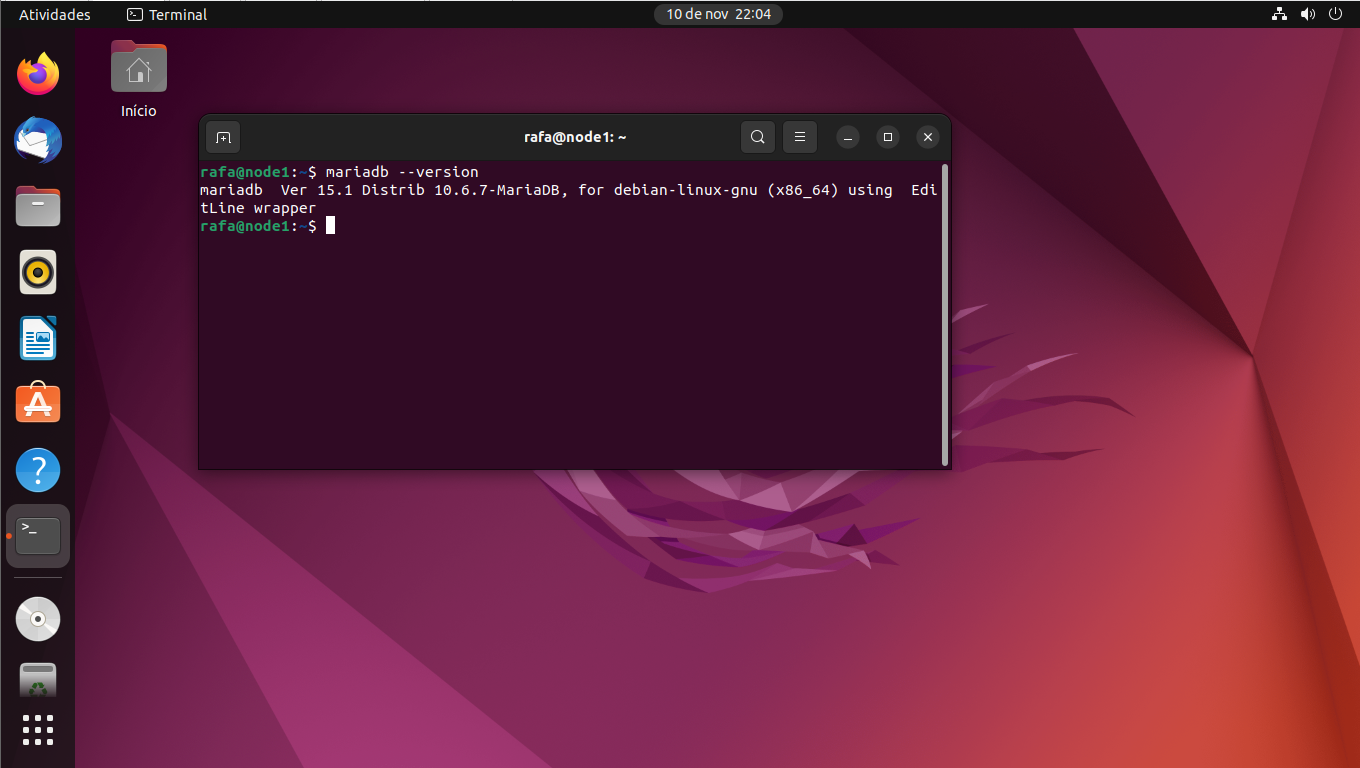
\includegraphics[width=13cm]{imagens/mariaversion.png}
\caption{Vesão mariadb}
\end{figure}

De seguida iniciar o serviço mariadb e configurar a inicialização automática quando se liga a \ac{VM}:

\begin{verbatim} sudo systemctl start mariadb \end{verbatim}

\begin{verbatim} sudo systemctl enable mariadb \end{verbatim}

\newpage
Verificar o estado "status" do mariadb:

\begin{verbatim} sudo systemctl status mariadb \end{verbatim}

\begin{figure}[H]
\center
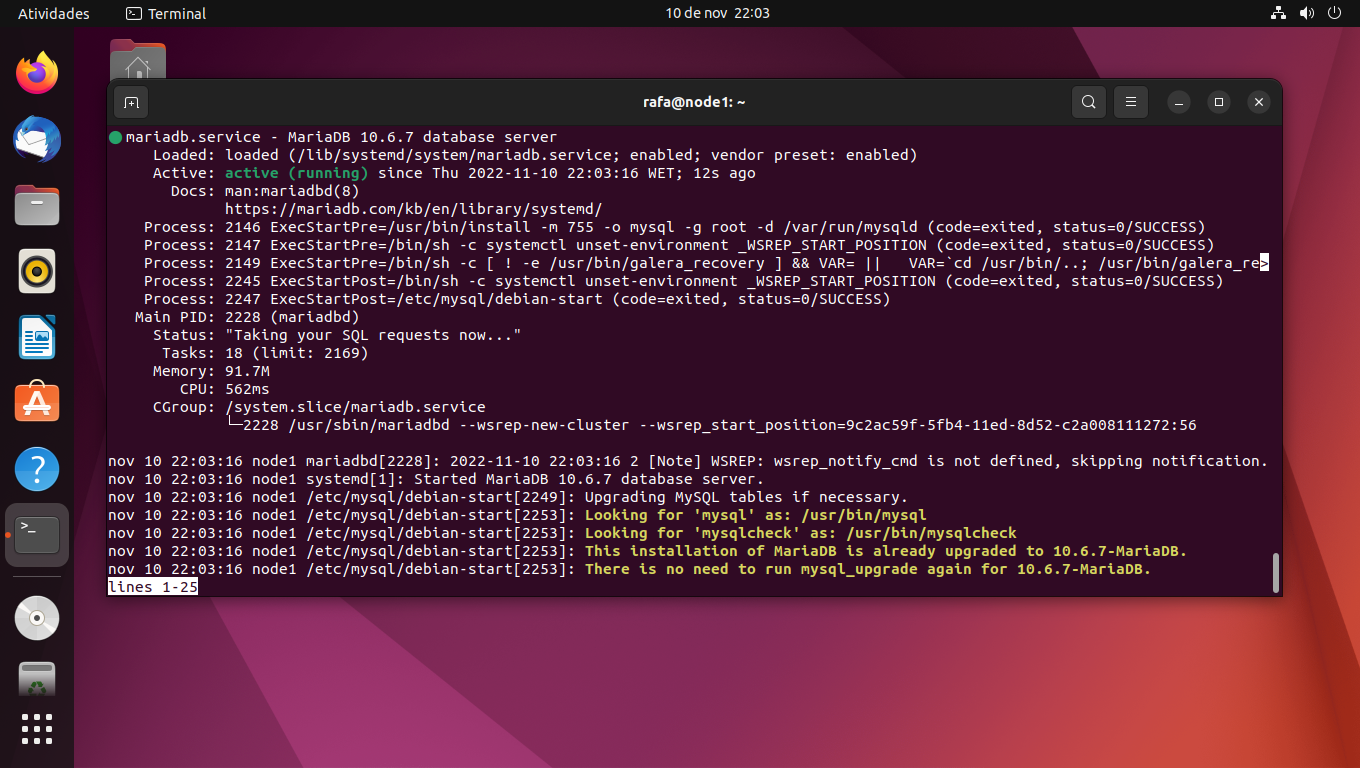
\includegraphics[width=13cm]{statusmaria.png}
\caption{Status mariaDB}
\end{figure}

Próximo passo é garantir a segurança mínima do serviço e para isso foi usado o seguinte comando:

\begin{verbatim} sudo mysql_secure_installation \end{verbatim}

Durante a nova configuração apenas é preciso aceitar todas as opções digitando, YES, e introduzir uma password.

De seguida, criamos uma nova conta de utilizador no servidor de \ac{BD} com autenticação e posteriormente atribuir privilégios administrativos a esse utilizador. Para isso entramos da seguinte forma:

\begin{verbatim} sudo mariadb -u root -p \end{verbatim}

\begin{figure}[H]
\center
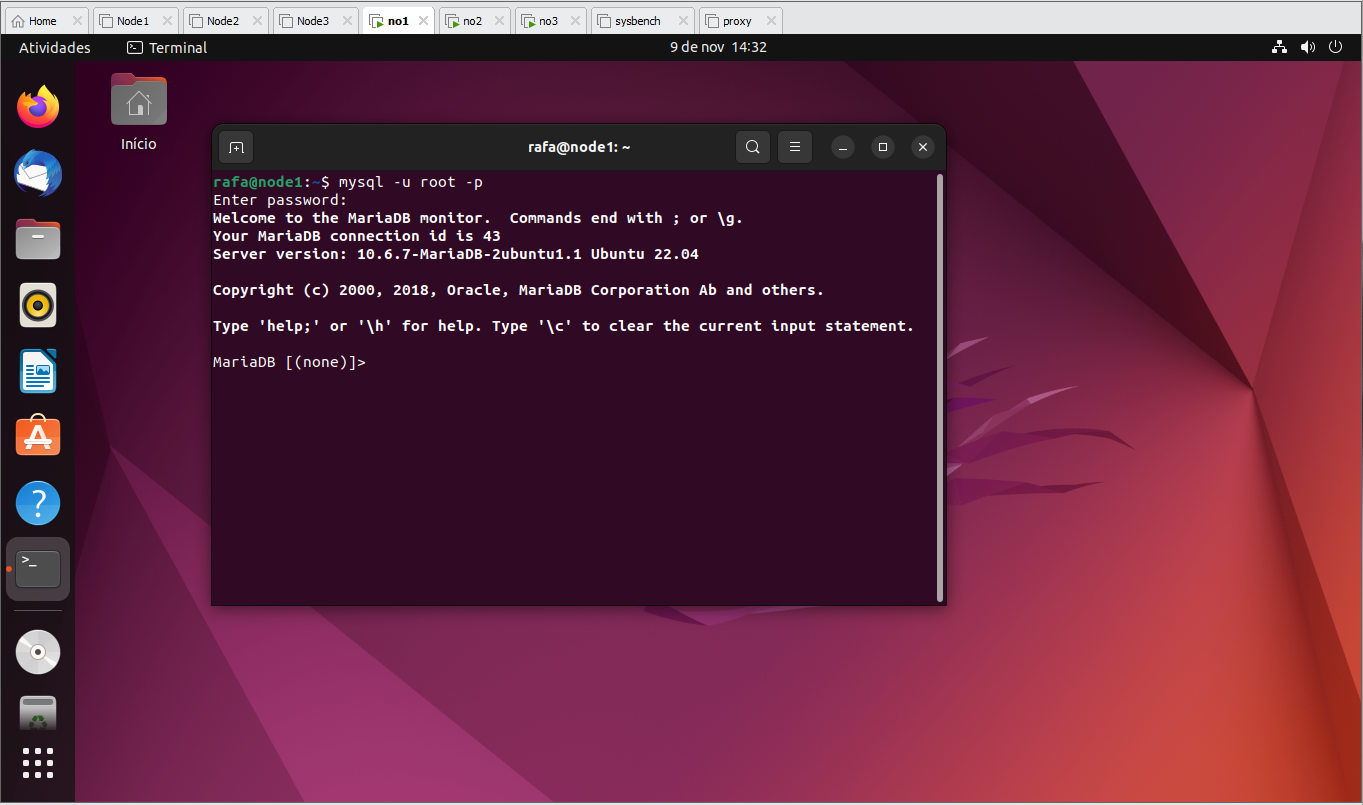
\includegraphics[width=13cm]{authmaria.png}
\caption{Login root Mysql}
\end{figure}

\newpage
Criar um utilizador com privilégios altos:

\begin{verbatim} CREATE USER 'admin_user'@'localhost' IDENTIFIED BY 'secret_password'; \end{verbatim}

NOTA: "admin\textunderscore user" será o nome do utilizador, e 'secret\textunderscore password' a password.

Privilégios:

\begin{verbatim} GRANT ALL PRIVILEGES ON *.* TO 'admin_user'@'localhost'; \end{verbatim}

NOTA: O *.* garante que o utilizador tem permissões para qualquer alteração ou inserção na base de dados.

Aplicar as alterações e de seguida sair.

\begin{verbatim} FLUSH PRIVILEGES; \end{verbatim}

\begin{verbatim} EXIT; \end{verbatim}

\newpage
\section{Configurar Galera Cluster}
Para que cada nó possa comunicar entre si precisamos de criar um arquivo de configuração Galera (repetir a criação do ficheiro galera nos vários nós):

\begin{verbatim} sudo nano /etc/mysql/conf.d/galera.cnf \end{verbatim}

Basta criar a seguinte configuração:
\begin{figure}[H]
\center
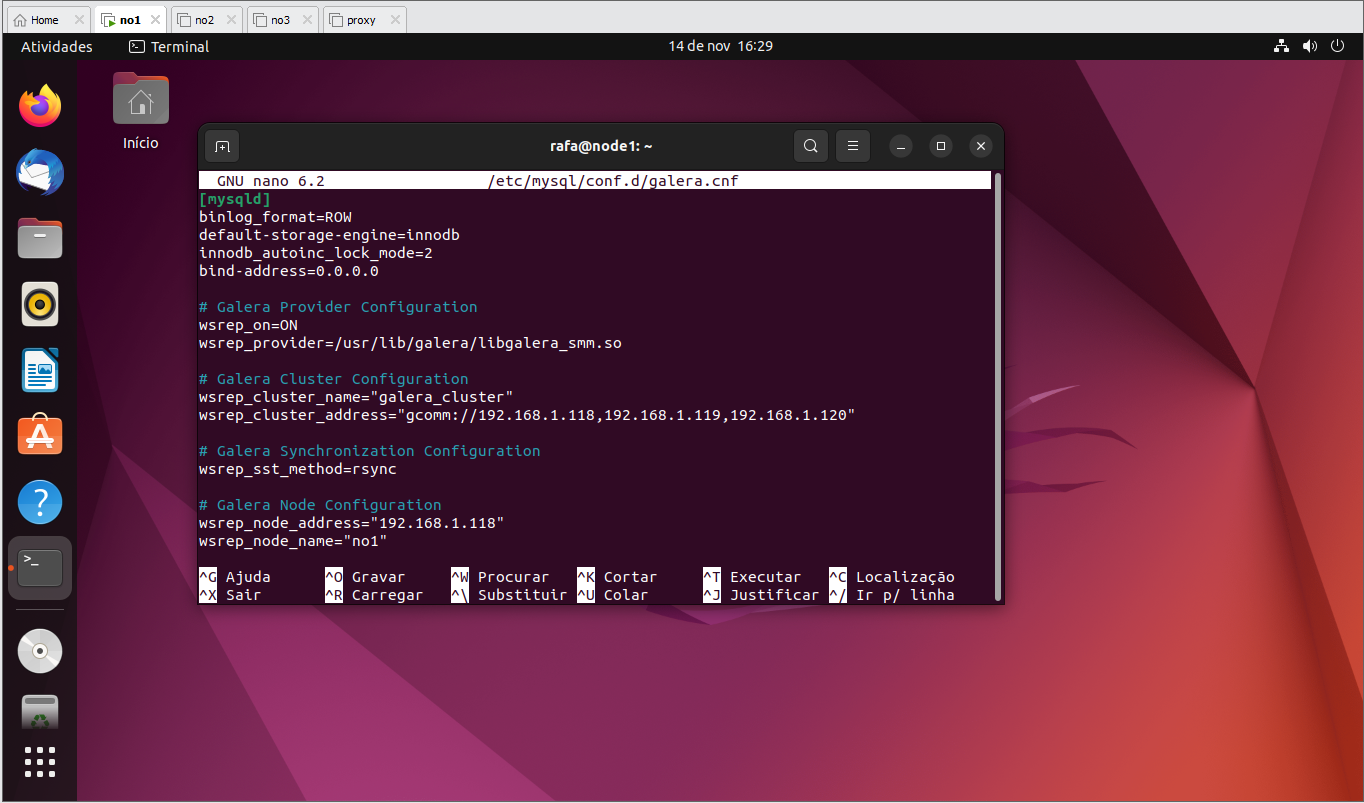
\includegraphics[width=13cm]{conf_galera.png}
\caption{Ficheiro Configuração Galera}
\end{figure}

Nos restantes nós apenas se altera o IP do "wsrep\textunderscore node\textunderscore address" e "wsrep\textunderscore node\textunderscore name".

\section{Iniciar o Galera Cluster}
Depois de concluir o passo anterior os nós estão preparados para comunicar uns com os outros.

De seguida, precisamos de interromper o serviço MariaDB em TODOS os nós.

\begin{verbatim} sudo systemctl stop mariadb \end{verbatim}

\begin{figure}[H]
\center
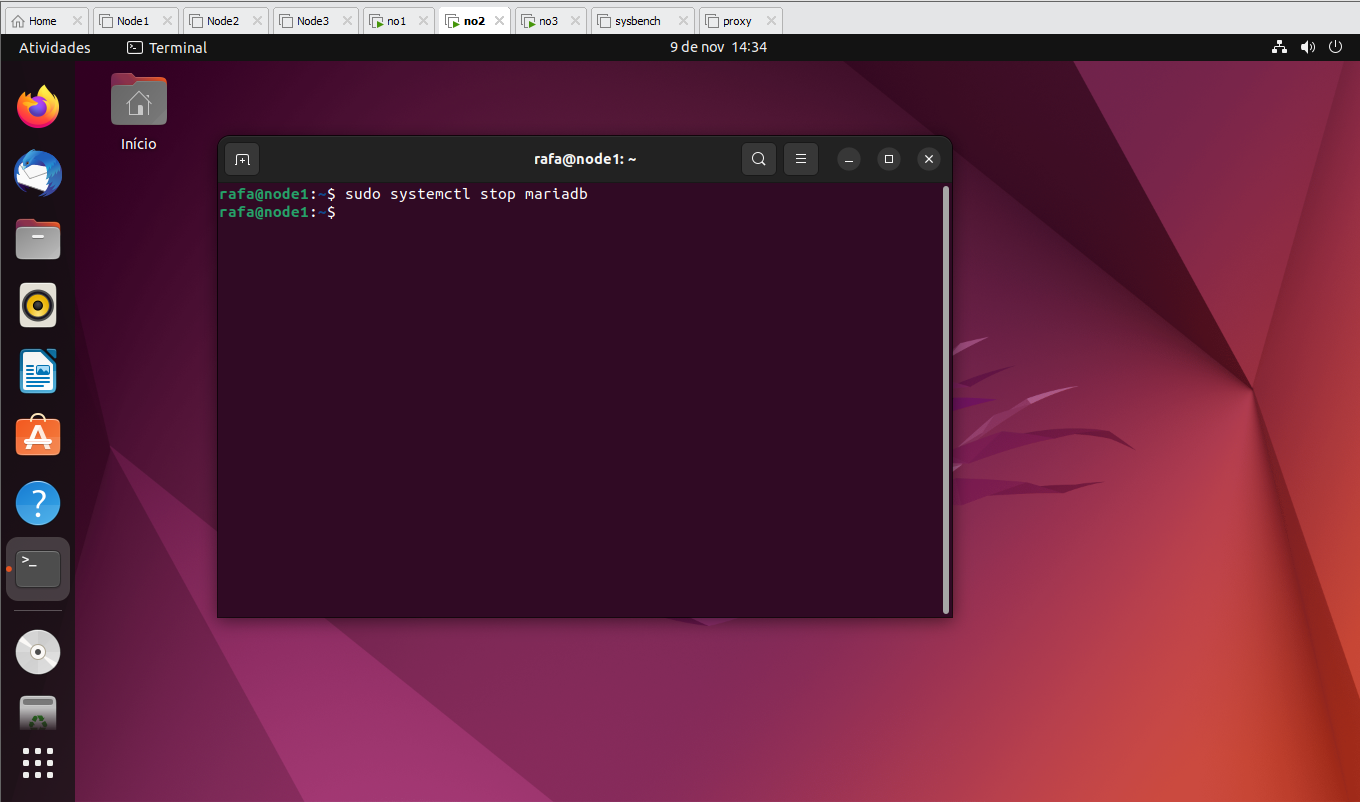
\includegraphics[width=13cm]{stopmaria.png}
\caption{STOP MariaDB}
\end{figure}

No primeiro nó, (de salientar que este comando é APENAS inserido no primeiro nó), o cluster MariaDB Galera é iniciado com o seguinte comando:

\begin{verbatim} galera_new_cluster \end{verbatim}

Agora, para verificar o tamanho do cluster entra-se como \textit{root} e utiliza-se:

\begin{verbatim} mysql -u root -p \end{verbatim}

\begin{verbatim} show status like 'wsrep_cluster_size'; \end{verbatim}

\begin{figure}[H]
\center
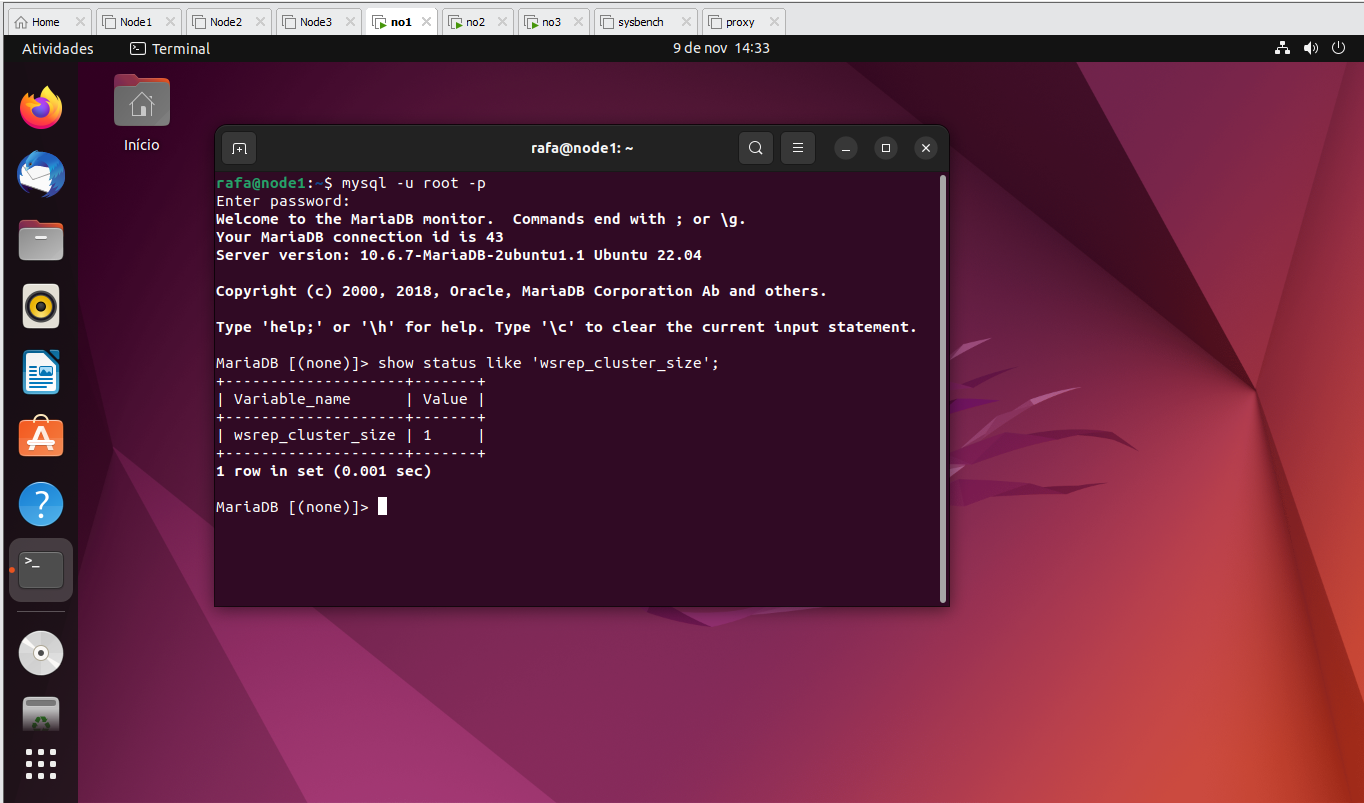
\includegraphics[width=13cm]{imagens/Screenshot_66.png}
\caption{Tamanho do cluster no nó 1}
\end{figure}

Ainda podemos verificar se o nó 1 tem conectividade com os restantes nós:

\begin{verbatim} SHOW GLOBAL STATUS LIKE 'wsrep_connected'; \end{verbatim}

\begin{figure}[H]
\center
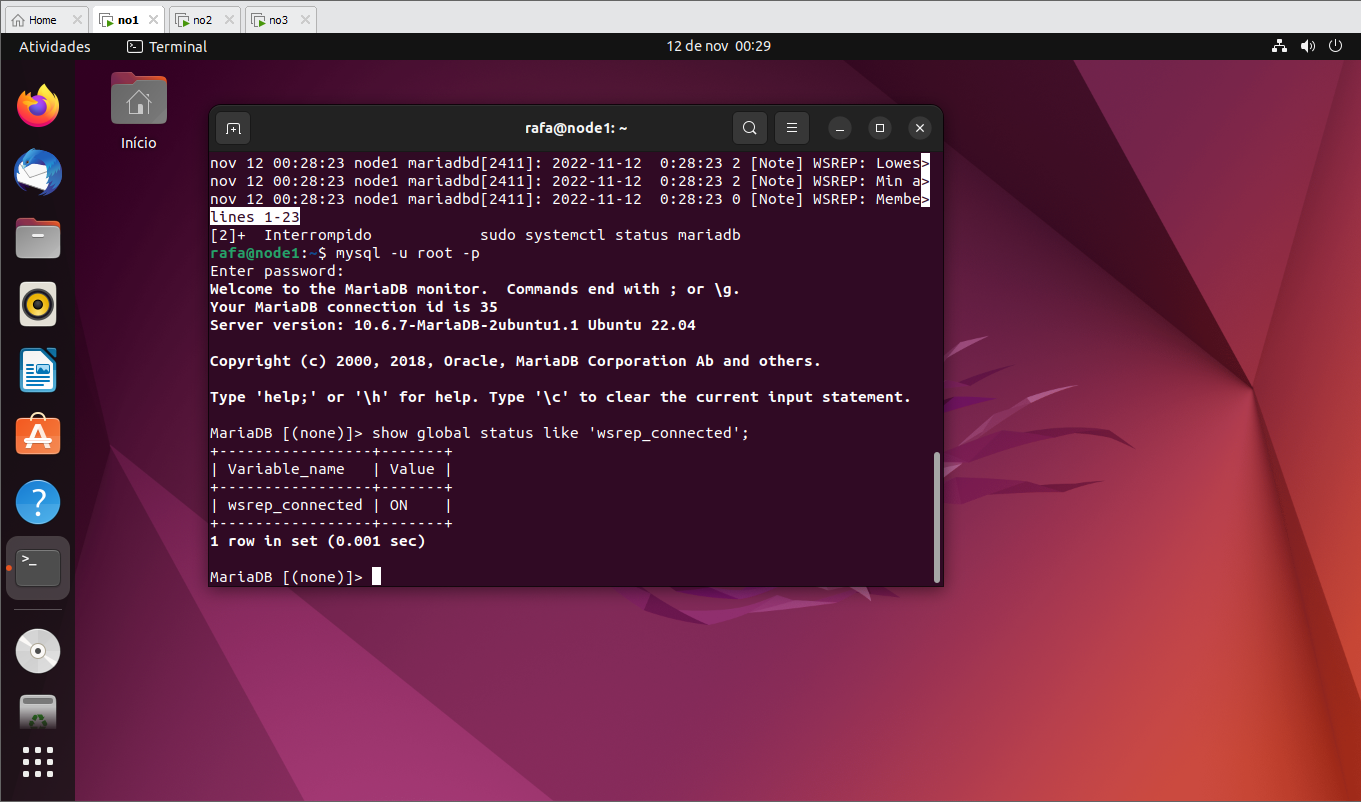
\includegraphics[width=13cm]{conectnodes.png}
\caption{Conectividade entre nós do cluster}
\end{figure}

No segundo nó, inicia-se o serviço MariaDB:

\begin{verbatim} systemctl start mariadb \end{verbatim}

\begin{figure}[H]
\center
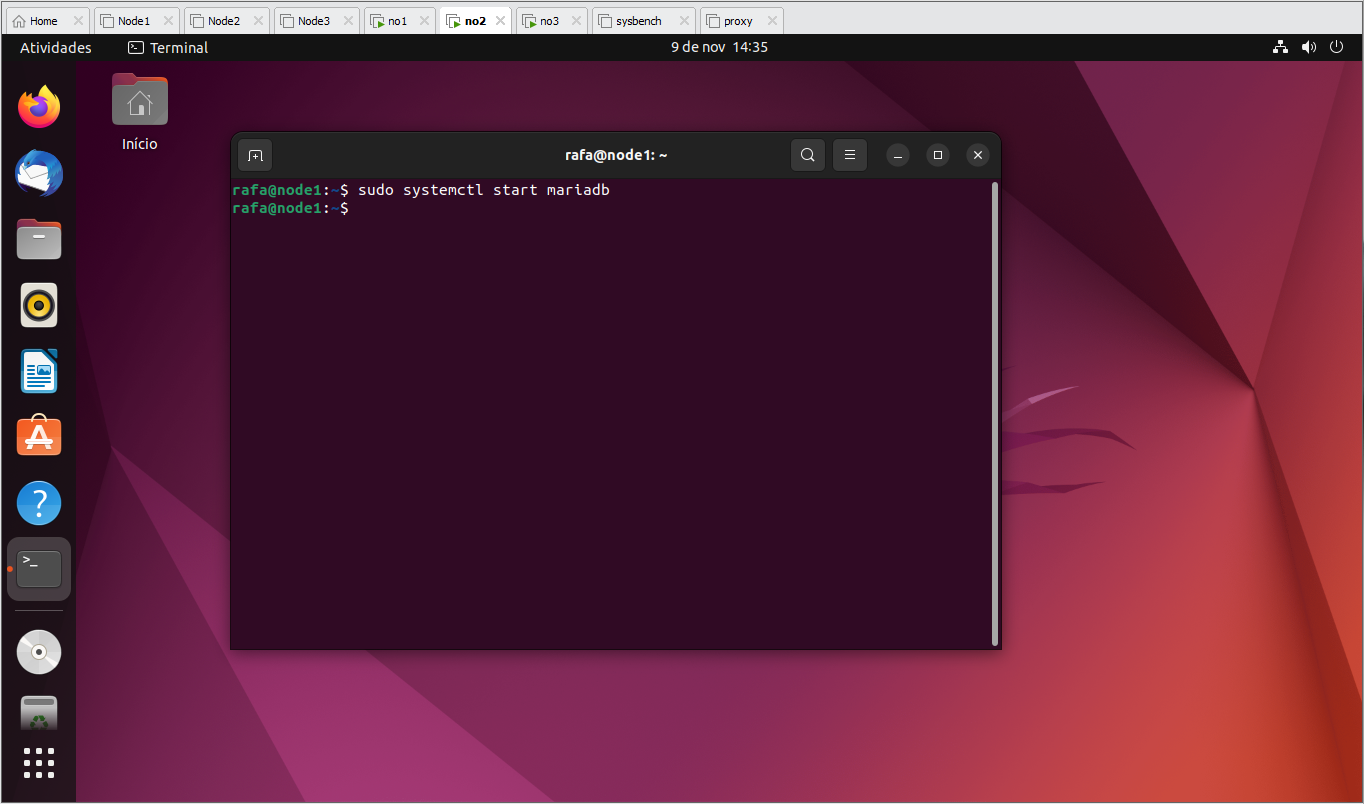
\includegraphics[width=13cm]{Screenshot_69.png}
\caption{START Cluster Nó 2}
\end{figure}

Repete-se o procedimento no segundo nó para verificar o tamanho do cluster:

\begin{verbatim} mysql -u root -p \end{verbatim}

\begin{verbatim} show status like 'wsrep_cluster_size'; \end{verbatim}

\begin{figure}[H]
\center
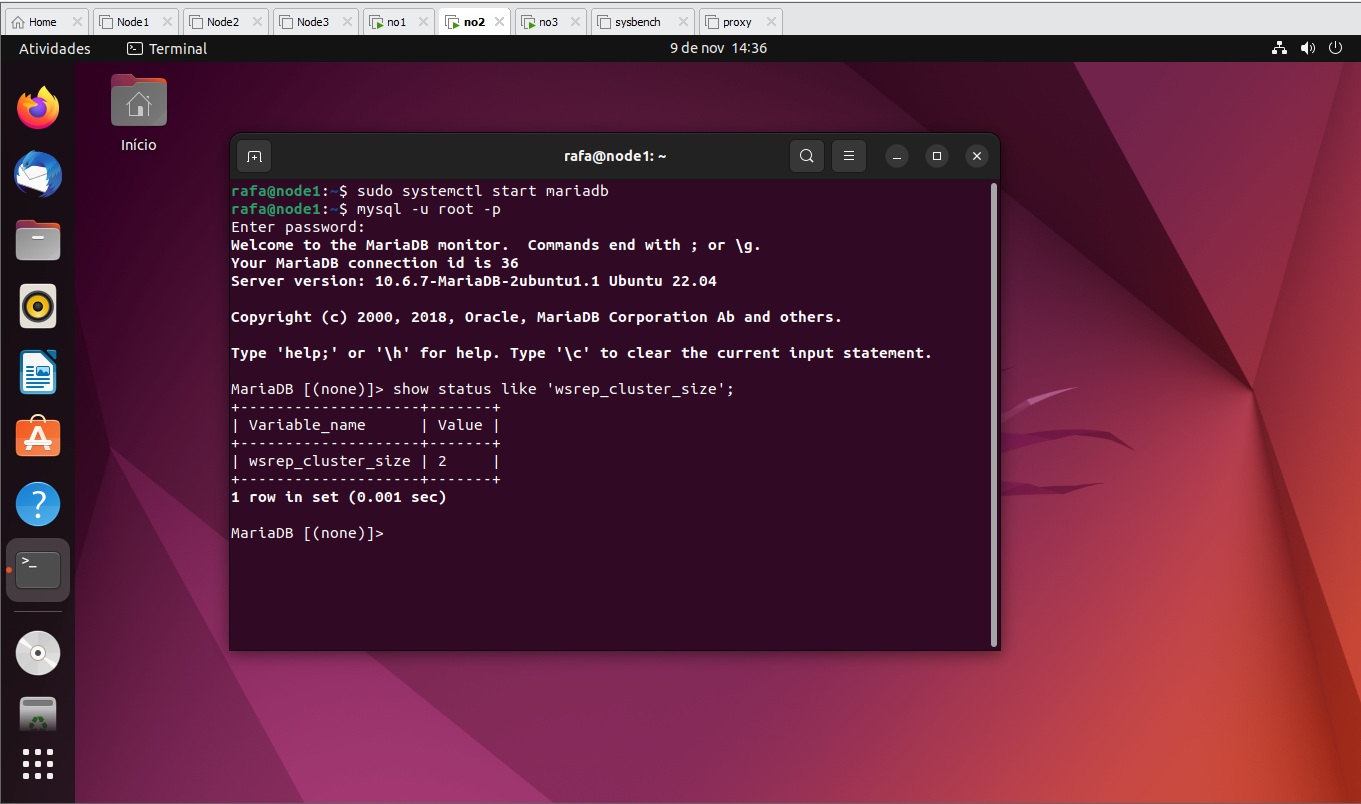
\includegraphics[width=13cm]{Screenshot_71.png}
\caption{Tamanho do cluster no nó 2}
\end{figure}

\newpage
Entretanto se verificar-mos o tamanho do cluster no nó 1, verificamos que o nó 1 e nó 2 já pertencem ao mesmo cluster galera:

\begin{figure}[H]
\center
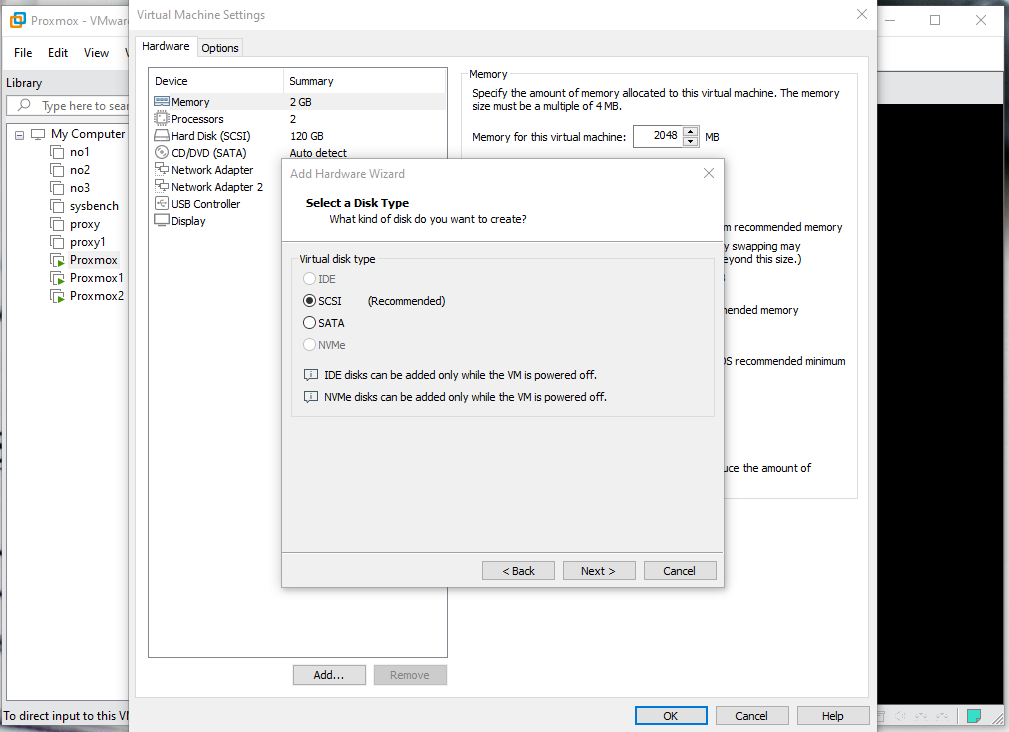
\includegraphics[width=13cm]{Screenshot_70.png}
\caption{Tamanho do cluster no nó 1}
\end{figure}

No terceiro nó, inicia-se o serviço MariaDB:

\begin{verbatim} systemctl start mariadb\end{verbatim}

\begin{figure}[H]
\center
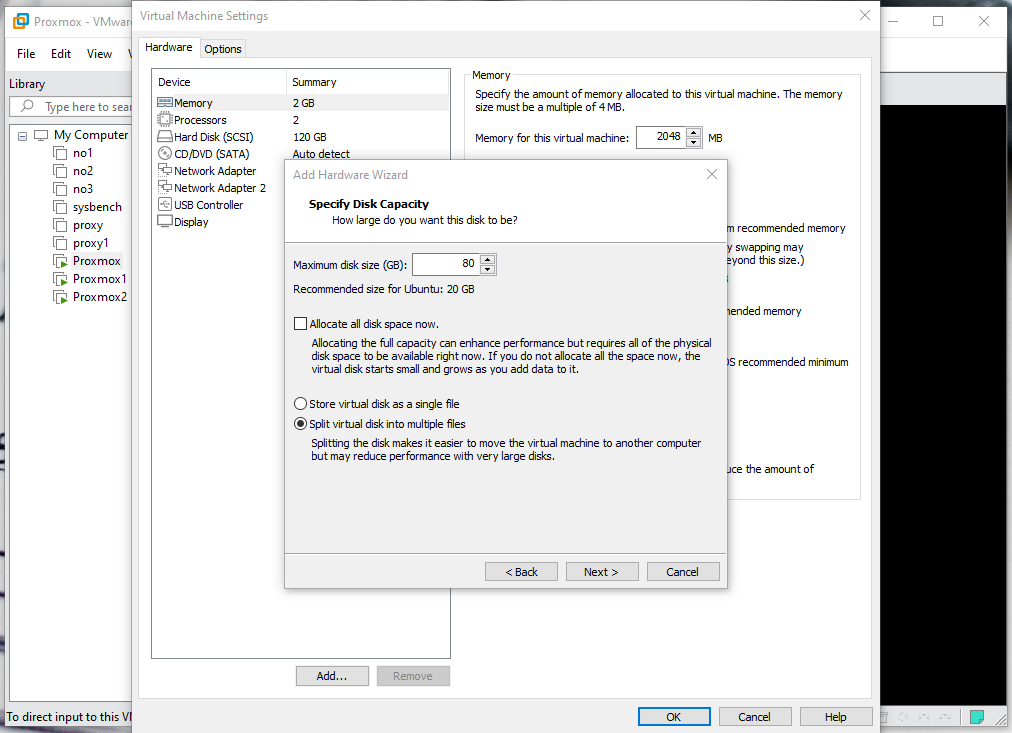
\includegraphics[width=13cm]{Screenshot_72.png}
\caption{START Cluster nó 3}
\end{figure}

\newpage
Repete-se o procedimento no segundo nó para verificar o tamanho do cluster:

\begin{verbatim} mysql -u root -p \end{verbatim}

\begin{verbatim} show status like 'wsrep_cluster_size'; \end{verbatim}

\begin{figure}[H]
\center
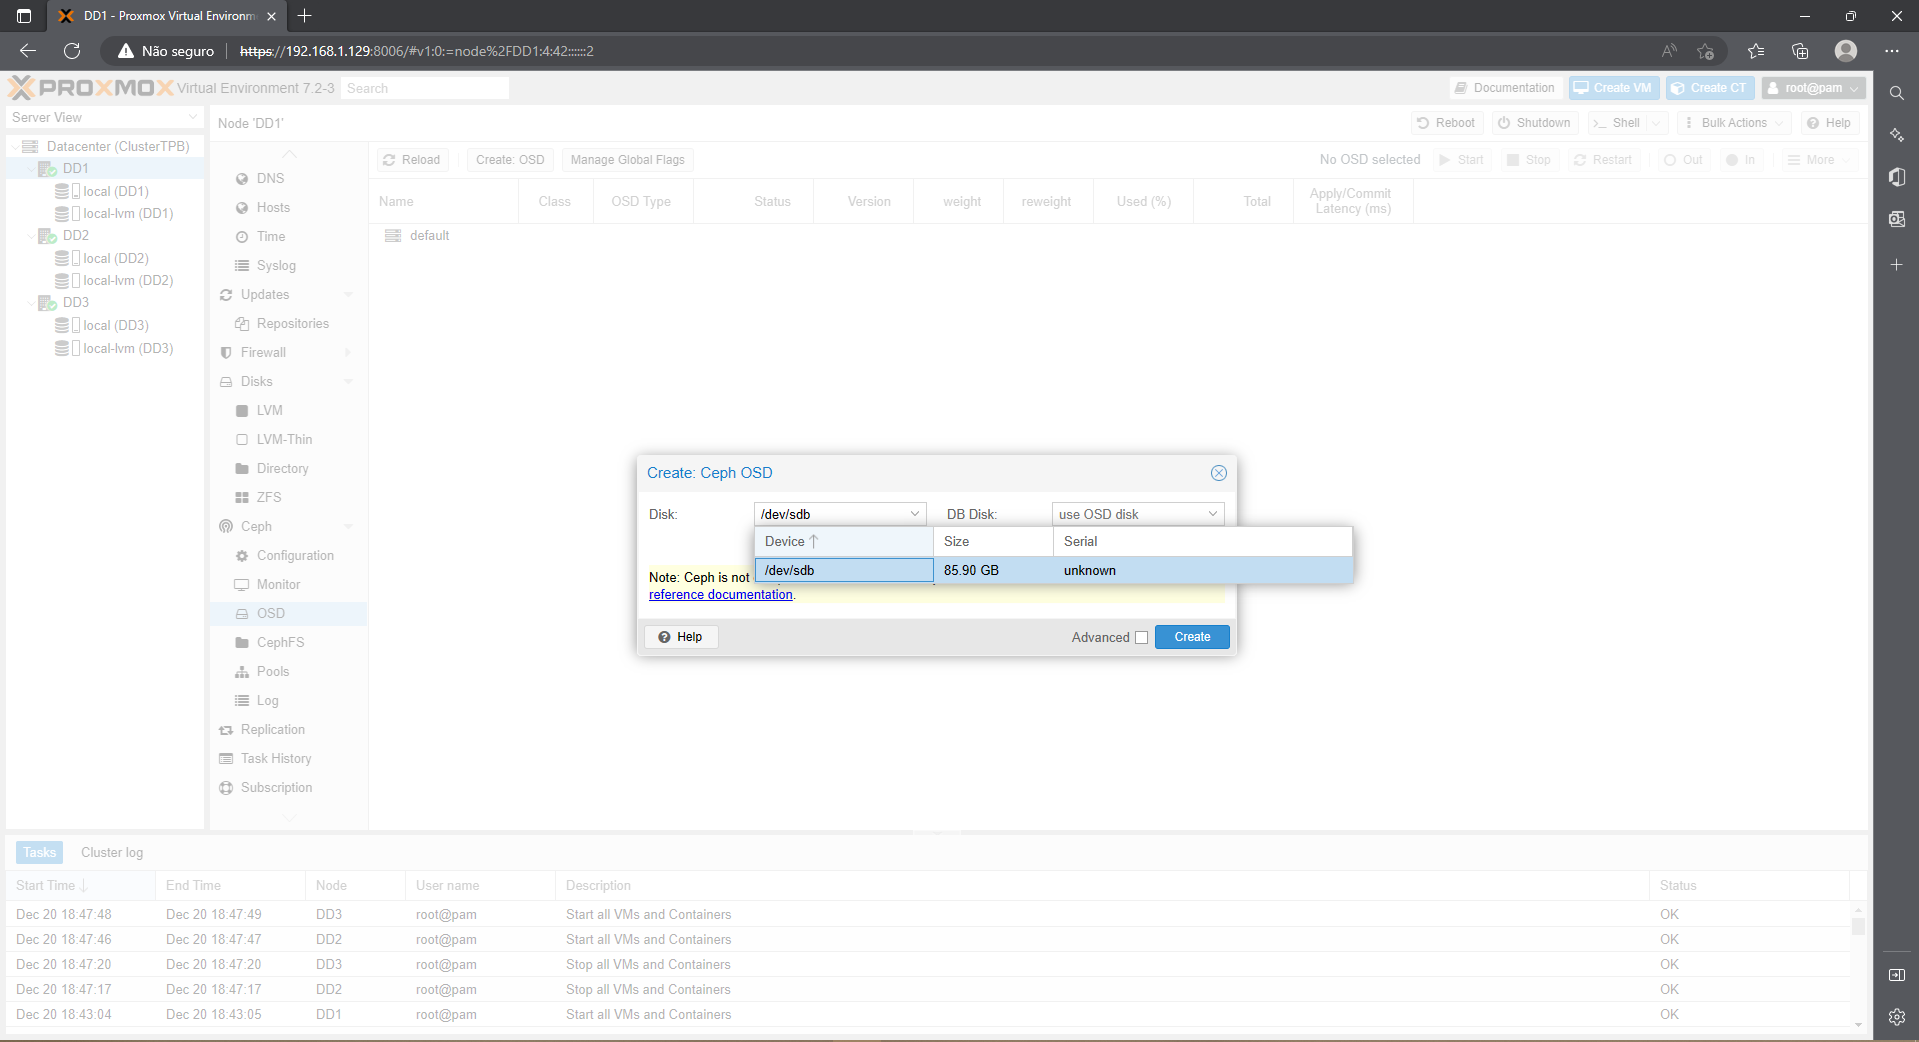
\includegraphics[width=13cm]{Screenshot_74.png}
\caption{Tamanho do cluster no nó 3}
\end{figure}

Entretanto se se verificar novamente o tamanho do cluster no nó 1 verificamos que todos os nós já pertencem ao mesmo cluster galera:

\begin{figure}[H]
\center
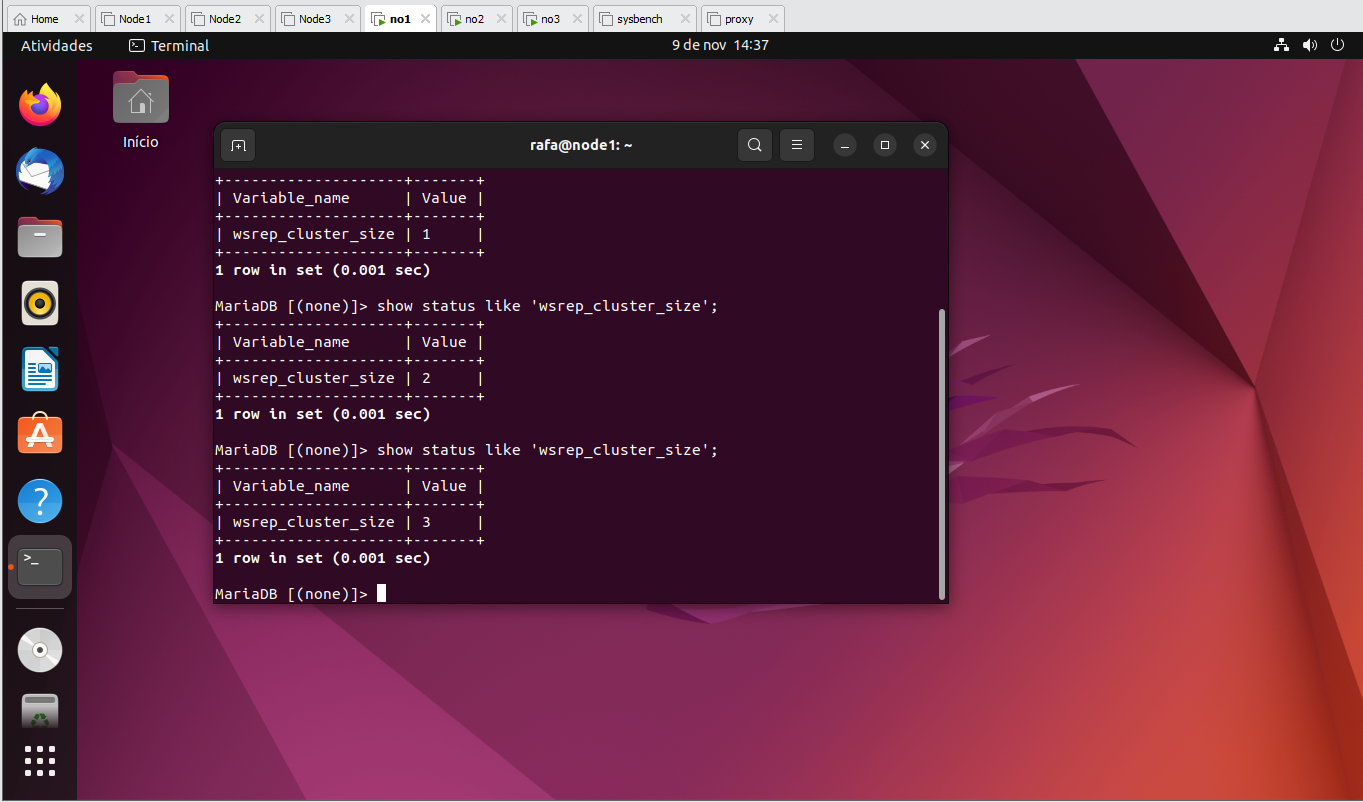
\includegraphics[width=13cm]{Screenshot_73.png}
\caption{Tamanho do cluster no nó 1}
\end{figure}

\newpage
\section{Replicação no Cluster}

Para testar a replicação com o cluster concluído (3 nós), criei uma base de dados no nó 1 para verificar se a mesma base de dados era replicada pelos restantes nós. 

Comecei por verificar as bases de dados existentes com o comando:

\begin{verbatim} SHOW DATABASES; \end{verbatim}

\begin{figure}[H]
\center
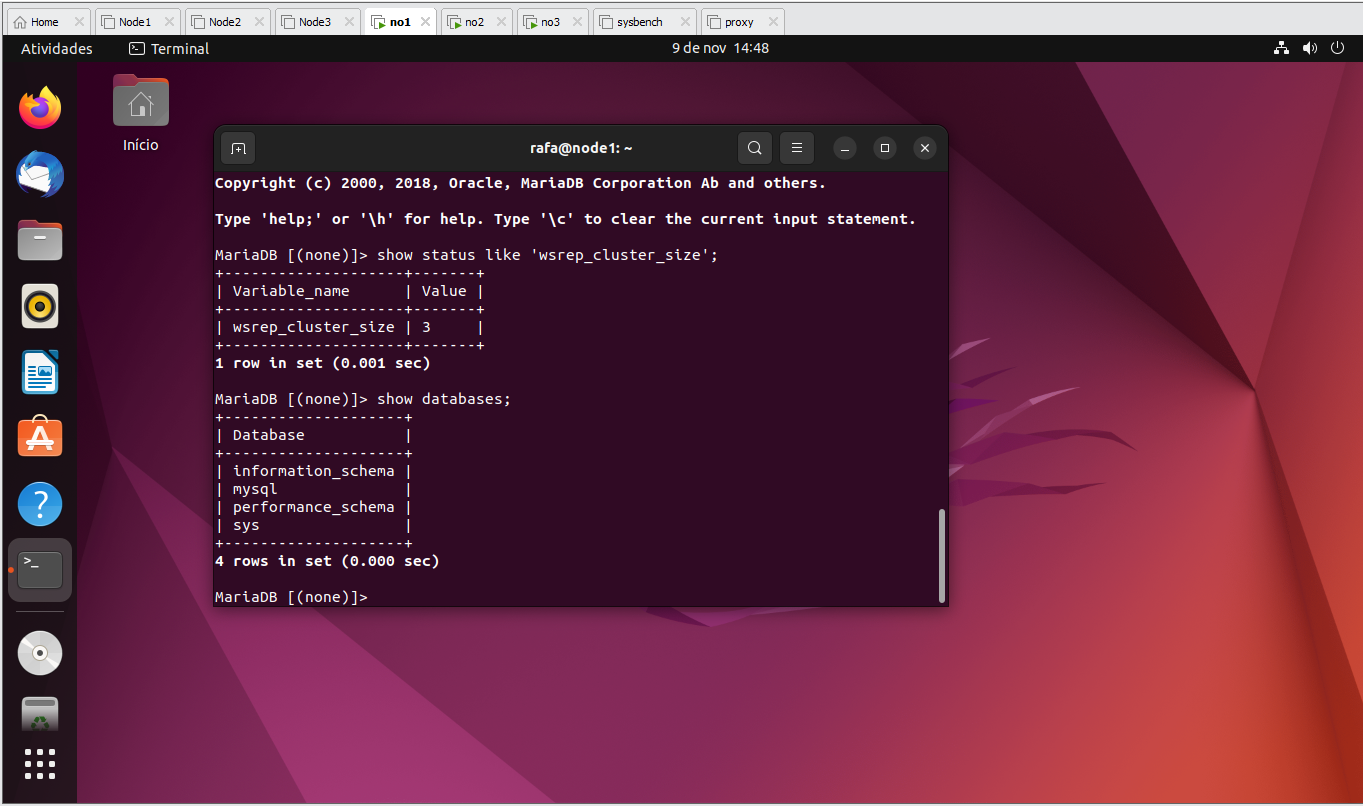
\includegraphics[width=13cm]{Screenshot_75.png}
\caption{Base de Dados existentes}
\end{figure}

De seguida, criei a base de dados e pude confirmar novamente com o comando \textit{ SHOW DATABASES;} que foi criada:

\begin{verbatim} CREATE DATABASE dbtest1; \end{verbatim}

\begin{figure}[H]
\center
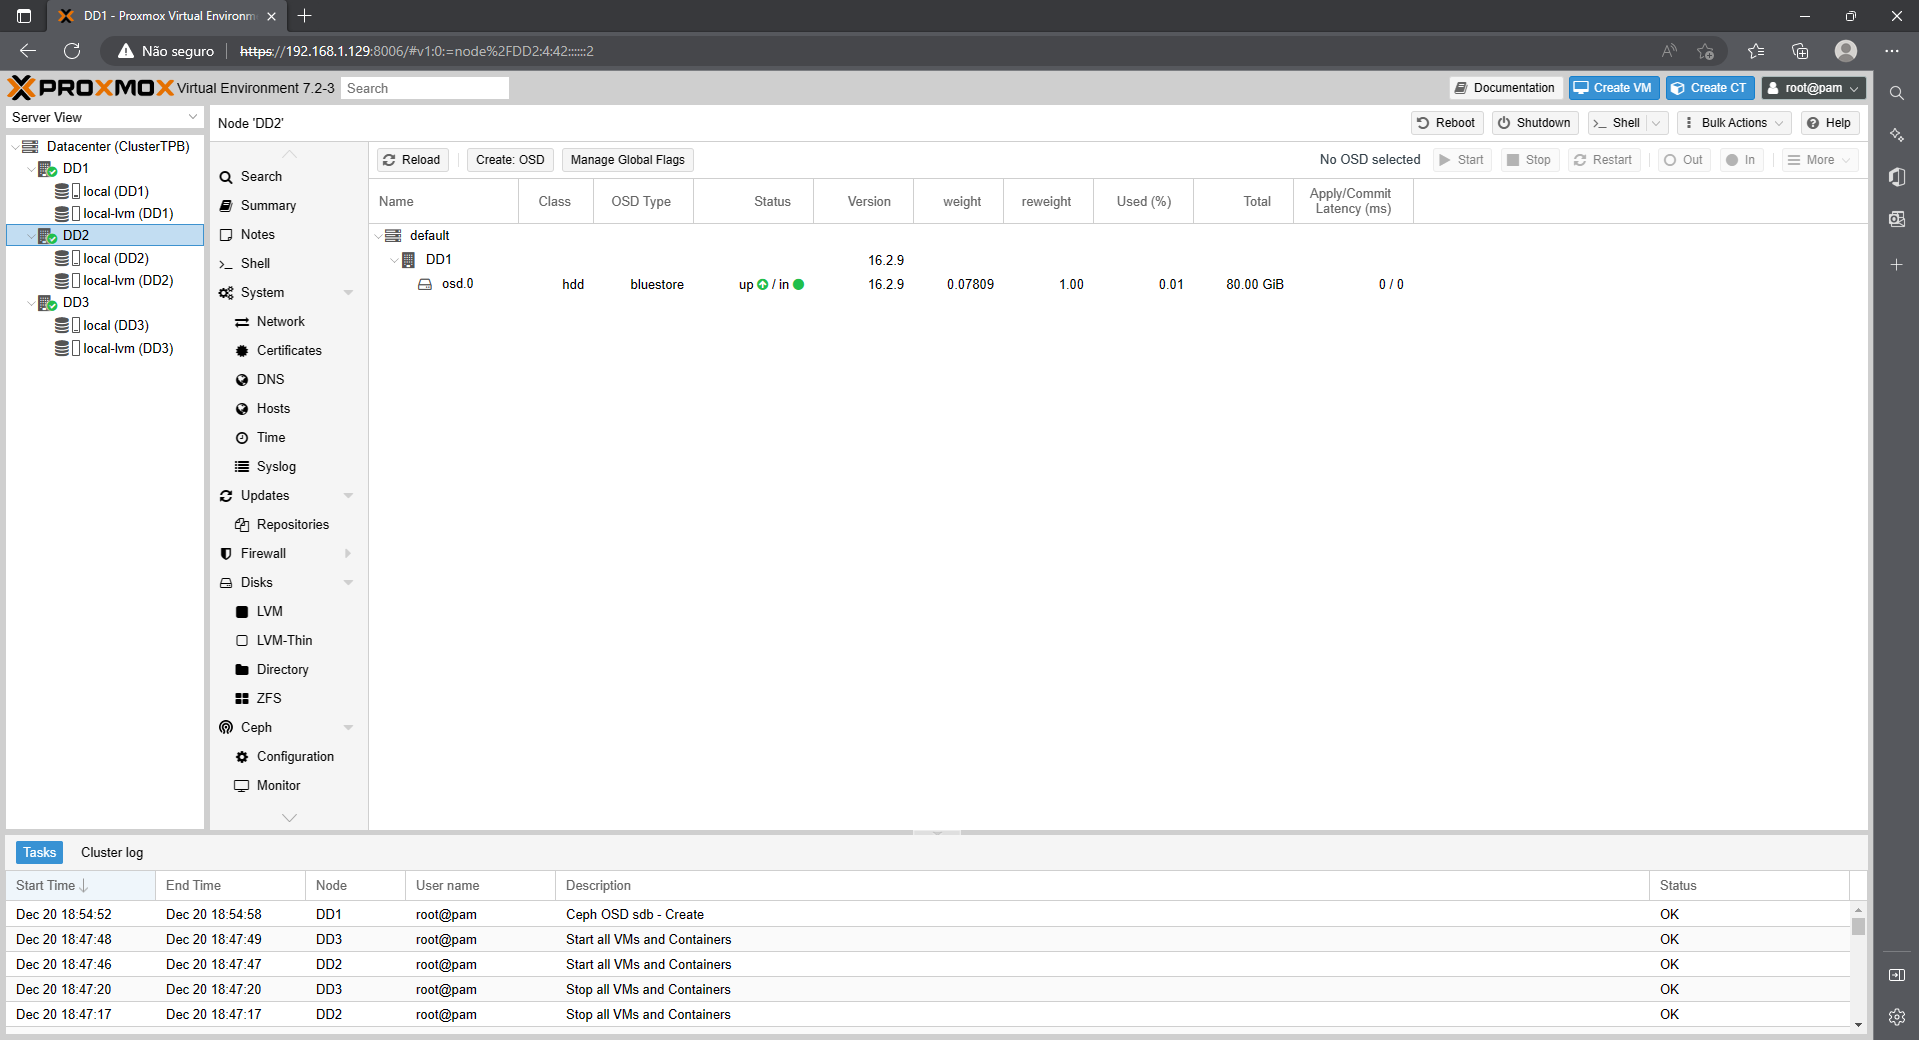
\includegraphics[width=13cm]{Screenshot_76.png}
\caption{Criação da Base de dados}
\end{figure}

\newpage
Passando para o nó 2 e 3 para verificar se a \ac{BD} criada já existe no cluster basta fazer \textit{login} no MariaDB como \textit{root} e verificar com os comandos acima já mencionados:

\begin{verbatim}SHOW DATABASES;\end{verbatim}

\begin{figure}[H]
\center
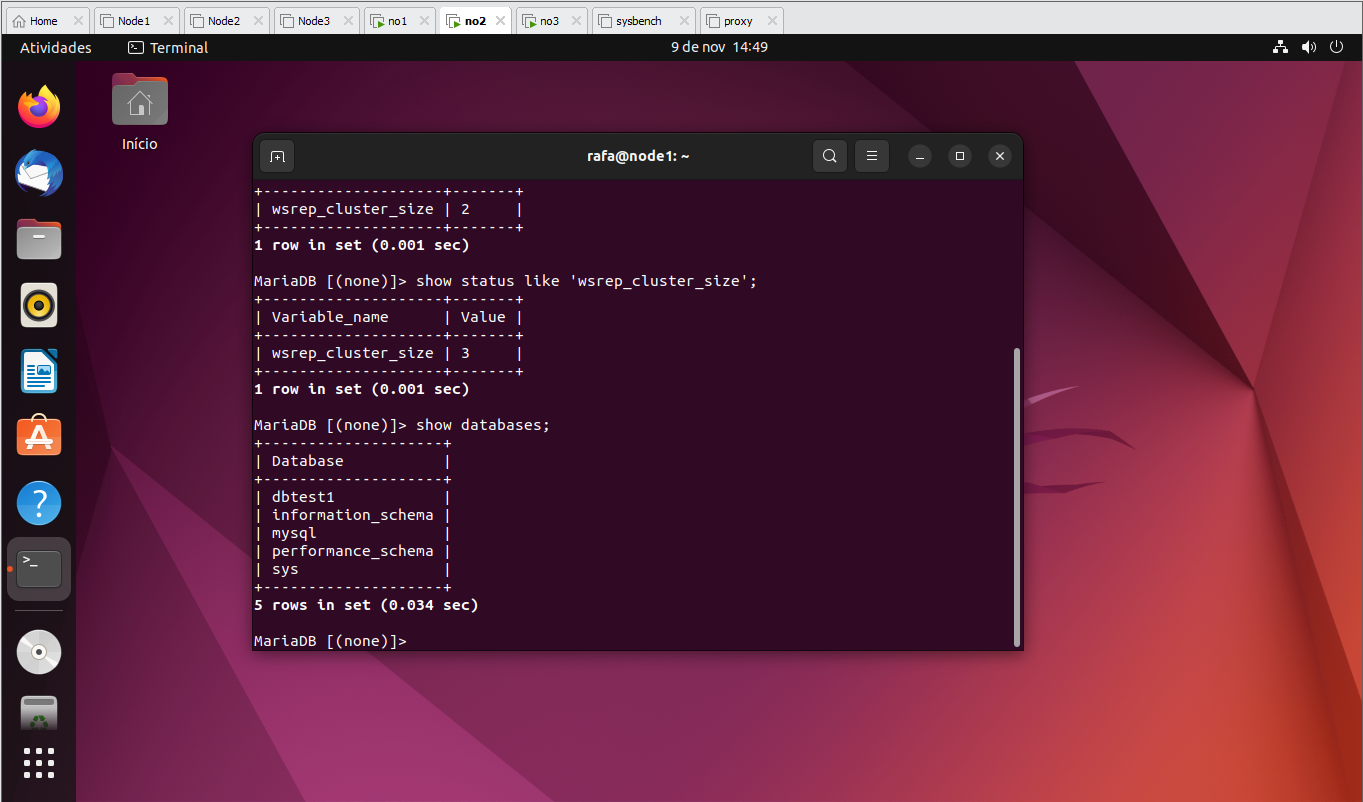
\includegraphics[width=13cm]{Screenshot_77.png}
\caption{Listagem \ac{BD}}
\end{figure}

Podemos verificar que a \ac{BD} \textit{dbtest1} inserida no nó 1 foi replicada de imediato para o nó 2 e para o 3:

\begin{figure}[H]
\center
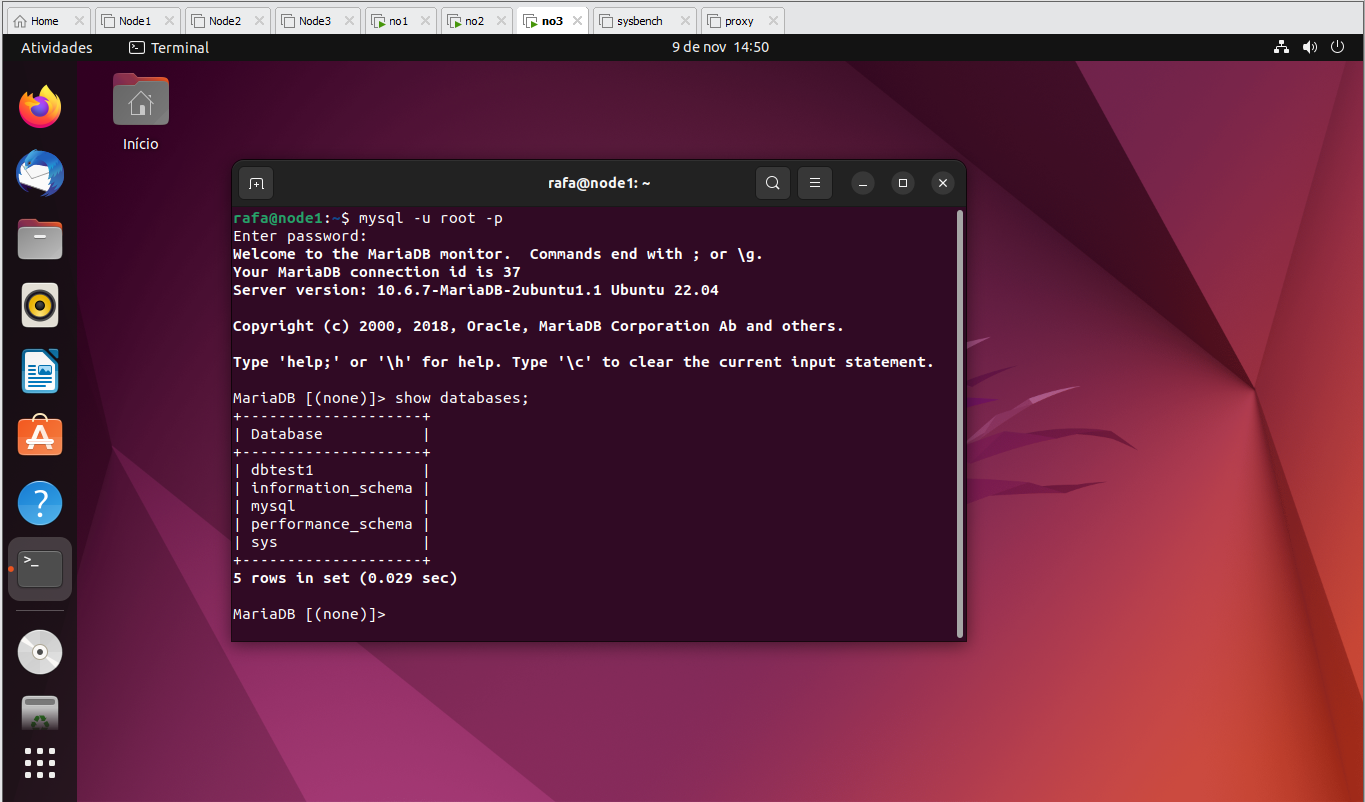
\includegraphics[width=13cm]{Screenshot_78.png}
\caption{Listagem \ac{BD}}
\end{figure}

\newpage
Por fim, ainda pude verificar as várias informações/definições gravadas no cluster:

\begin{verbatim}SHOW STATUS LIKE 'WSREP_\%';\end{verbatim}

\begin{figure}[H]
\center
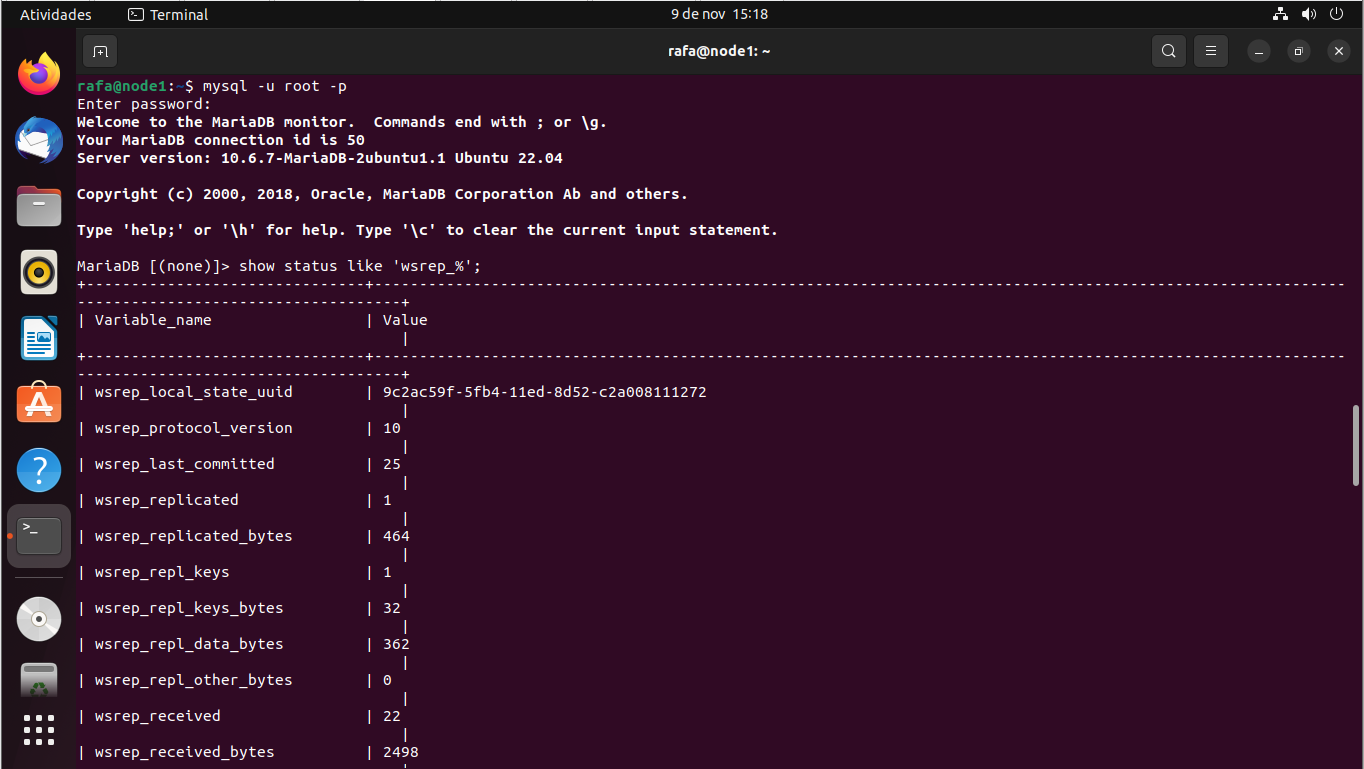
\includegraphics[width=13cm]{Screenshot_88.png}
\caption{Informações do Cluster}
\end{figure}

\begin{figure}[H]
\center
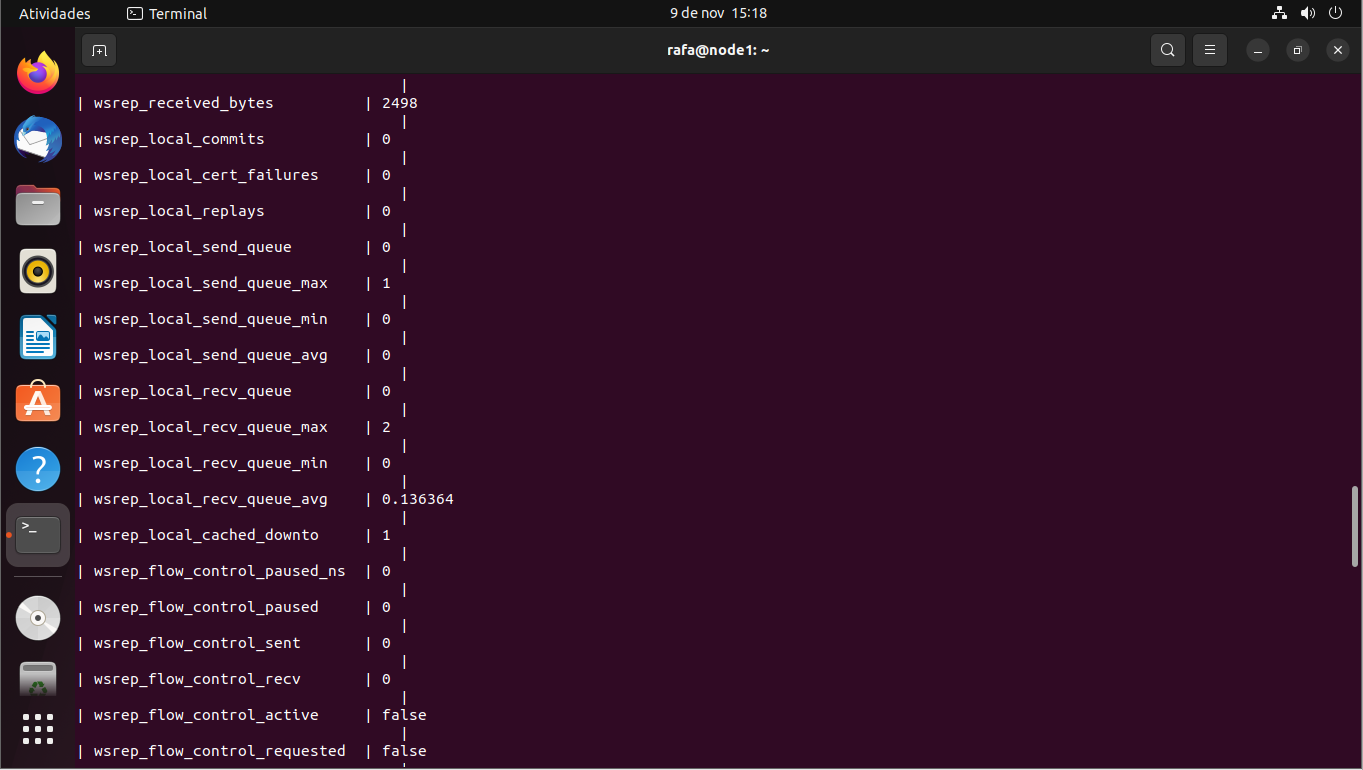
\includegraphics[width=13cm]{Screenshot_89.png}
\caption{Informações do Cluster}
\end{figure}

\begin{figure}[H]
\center
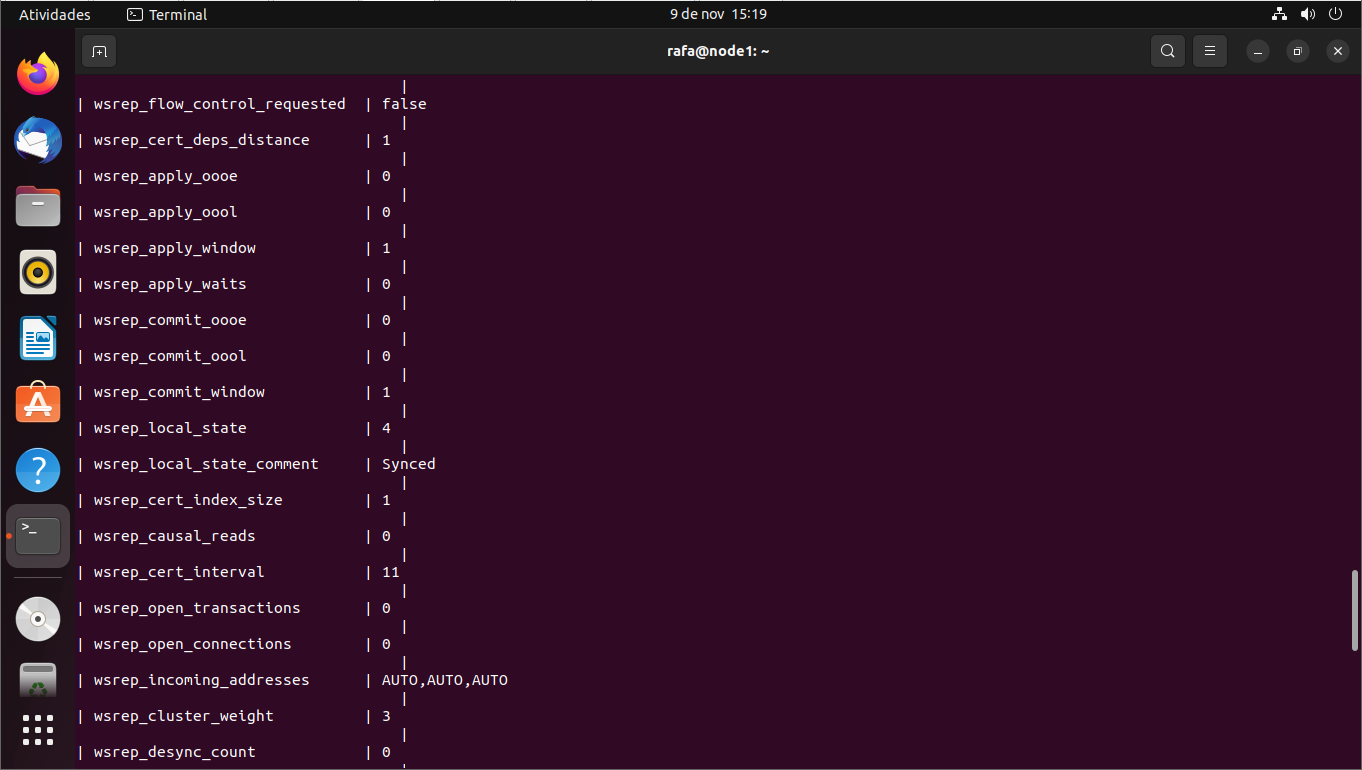
\includegraphics[width=13cm]{Screenshot_90.png}
\caption{Informações do Cluster}
\end{figure}

\begin{figure}[H]
\center
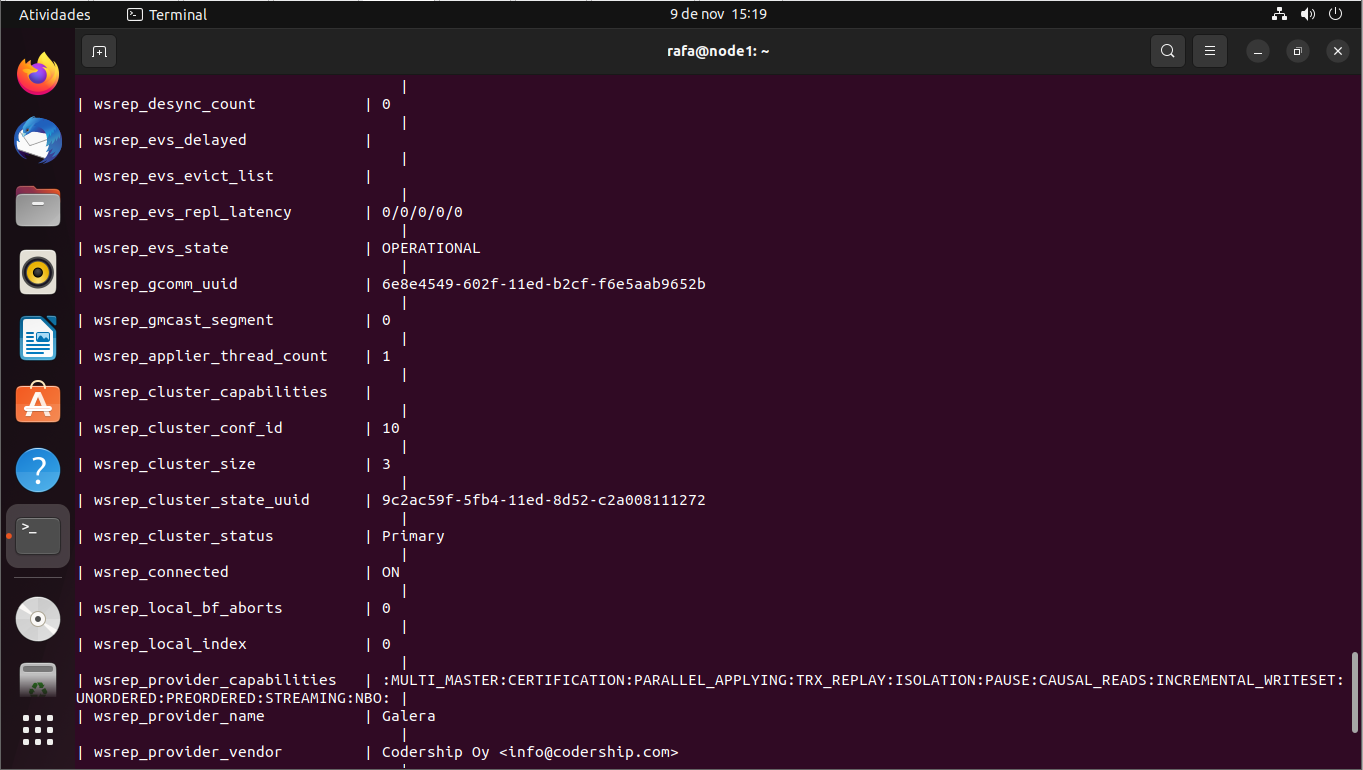
\includegraphics[width=13cm]{Screenshot_91.png}
\caption{Informações do Cluster}
\end{figure}

\begin{figure}[H]
\center
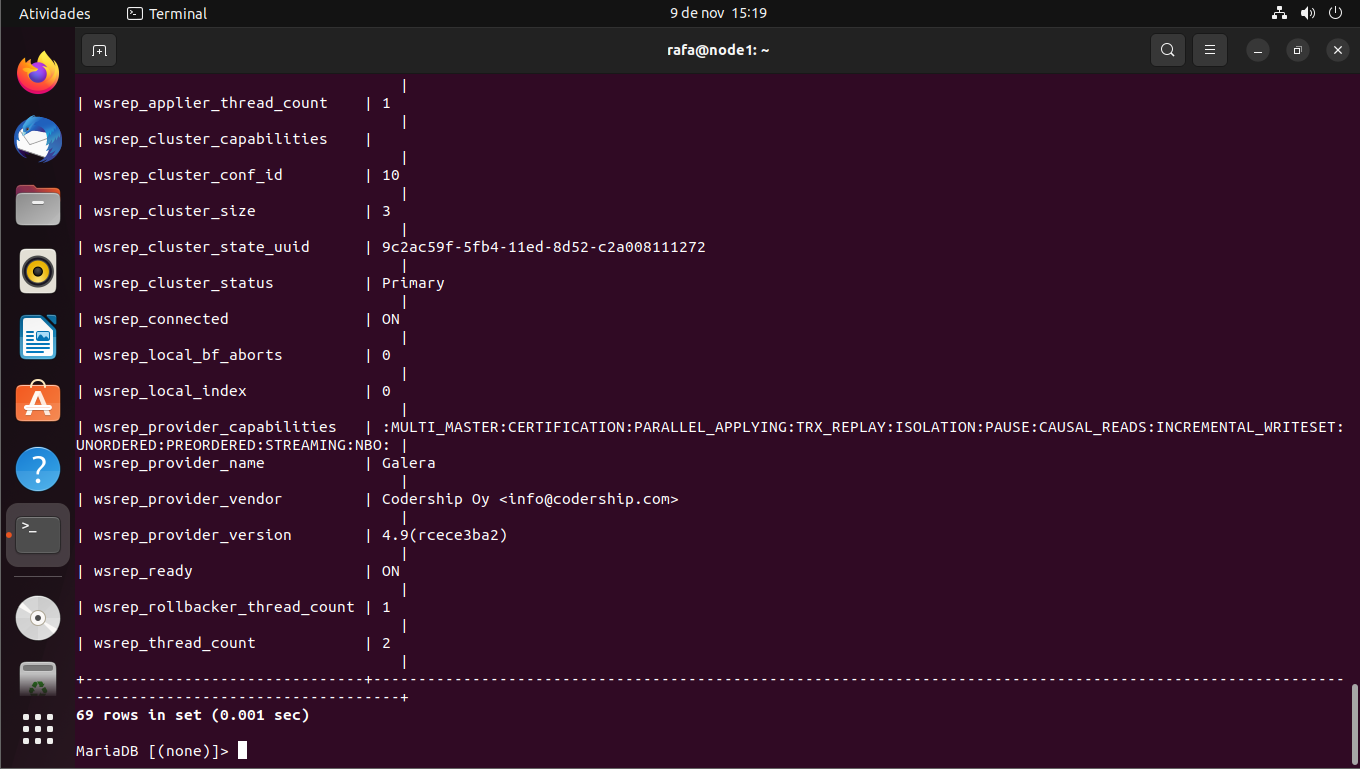
\includegraphics[width=13cm]{Screenshot_92.png}
\caption{Informações do Cluster}
\end{figure}


\section{Instalação e Configuração Galera Manager}
Para esta componente da meta 4, não consegui explorar devido ao fato de estar a usar o Ubuntu 22.04 e ser incompatível com o Galera Manger. Como prova fica anexado na figura abaixo.

\begin{figure}[H]
\center
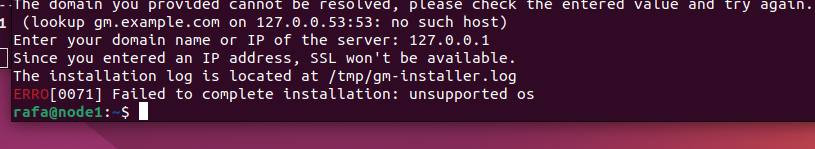
\includegraphics[width=13cm]{galera_manager.png}
\caption{Erro Galera Manager}
\end{figure}

\newpage
\section{Proxy}
Para executar este novo tema denominado como Proxy, foi adicionado uma nova \ac{VM} com a mesmas características dos nós acima referidos e procedi à instalação do ProxySQL.

Antes de começar a avançar com o proxySQL como já sabia que iria ser preciso definir o \textit{bind-address} de cada nó com o \ac{IP} atribuído pela placa de rede comecei por fazer essa atribuição:

\begin{verbatim}sudo nano/etc/mysql/mariadb.conf.d/50-server.cnf\end{verbatim}

\begin{figure}[H]
\center
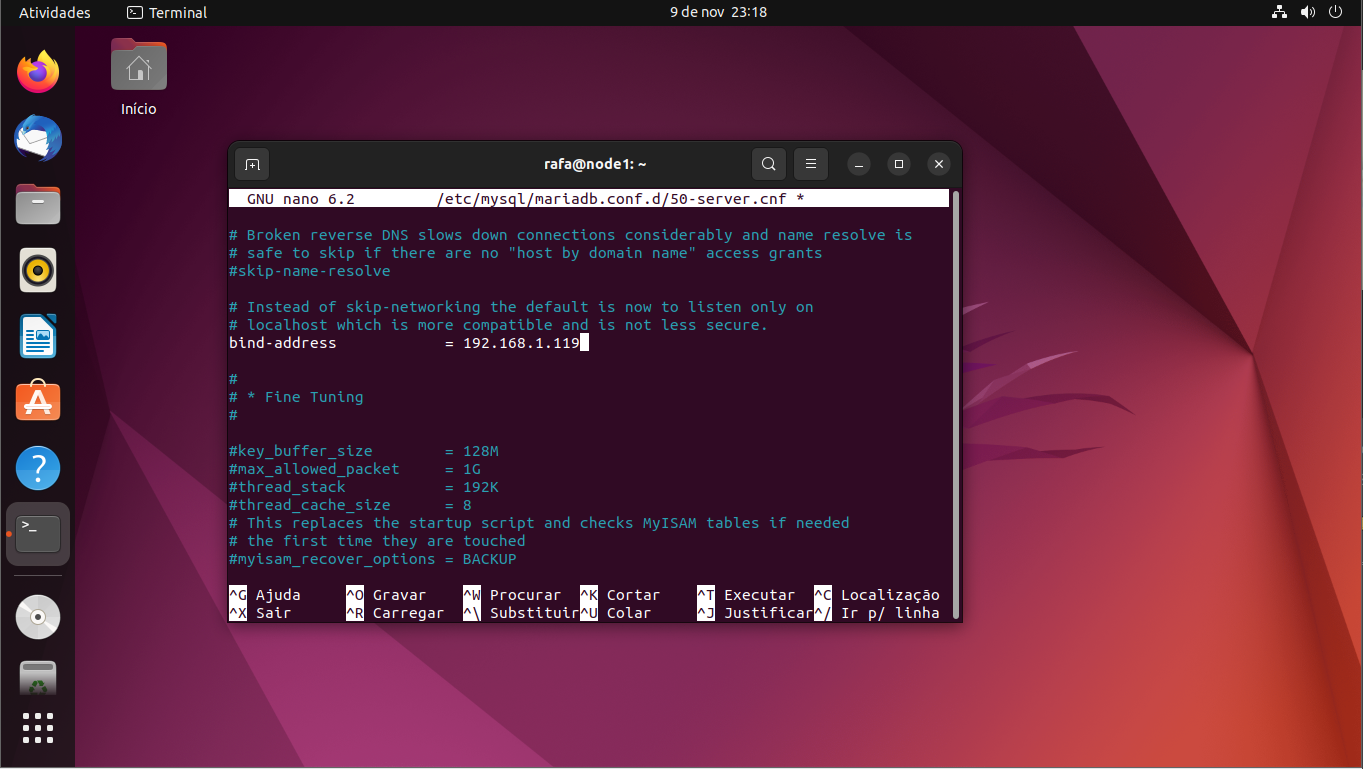
\includegraphics[width=13cm]{Screenshot_127.png}
\caption{Bind-Address Nós}
\end{figure}

\hfill \break
\indent Passo 1: Instalação ProxySQL
\begin{verbatim}wget https://github.com/sysown/proxysql/releases/download/v2.4.2/
proxysql_2.4.2-ubuntu20_amd64.deb \end{verbatim}

\begin{verbatim}dpkg -i proxysql_2.4.2-ubuntu20_amd64.deb \end{verbatim}

\begin{verbatim}sudo apt install mysql-client\end{verbatim}

Iniciar o serviço ProxySQL:
\begin{verbatim}sudo systemctl start proxysql\end{verbatim}

Habilitar o serviço ProxySQL no sistema:
\begin{verbatim}sudo systemctl enable --now proxysql\end{verbatim}

\newpage
Verificar o estado do serviço ProxySQL:
\begin{verbatim}sudo systemctl status proxysql\end{verbatim}

\begin{figure}[H]
\center
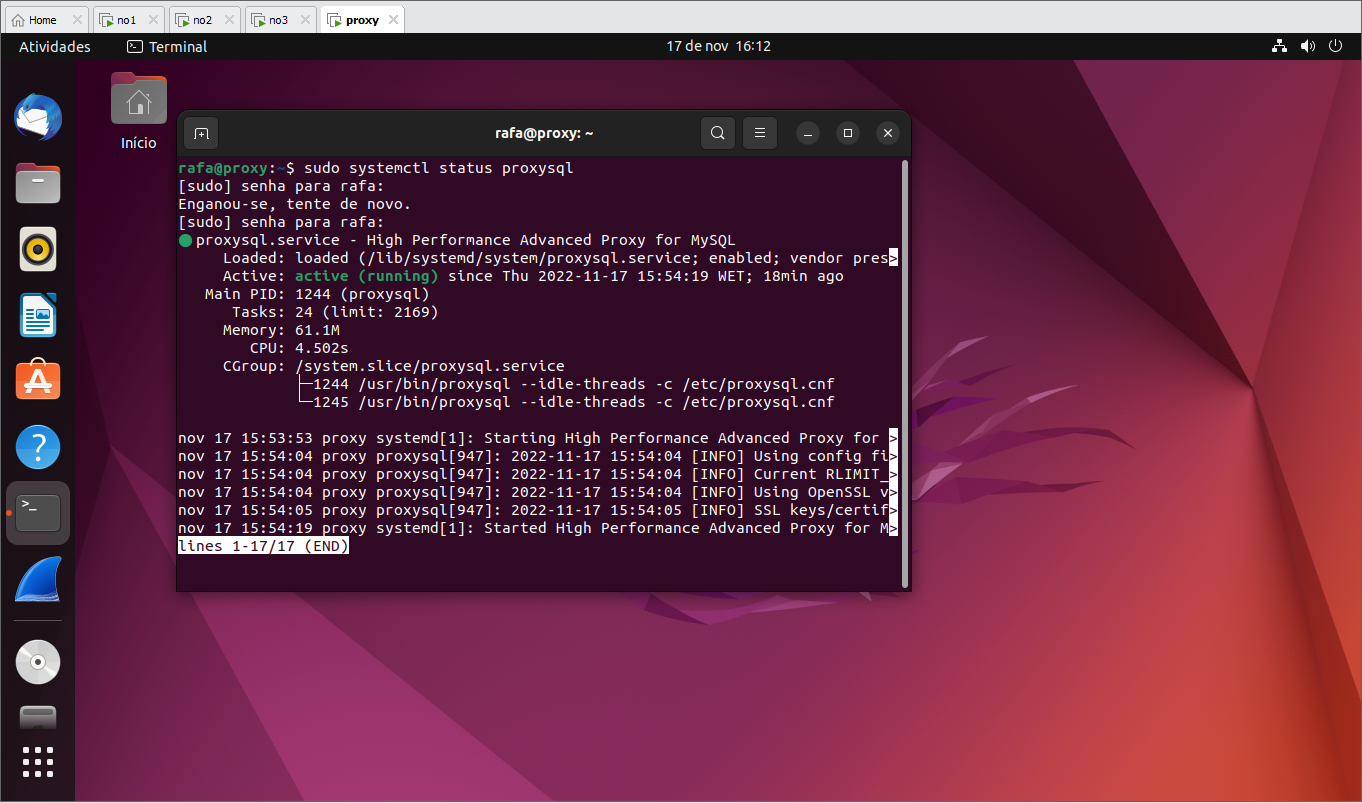
\includegraphics[width=13cm]{active_proxy.png}
\caption{STATUS ProxySQL}
\end{figure}

\hfill \break
\indent Passo 2: Configurar o ProxySQL

\hfill \break
\indent Para me conectar a área administrativa do ProxySQL foi preciso criar um cliente com a respetiva password:

\begin{verbatim}mysql -u admin -psenhasegura -h 127.0.0.1 -P6032 --prompt='Admin> '\end{verbatim}

\begin{figure}[H]
\center
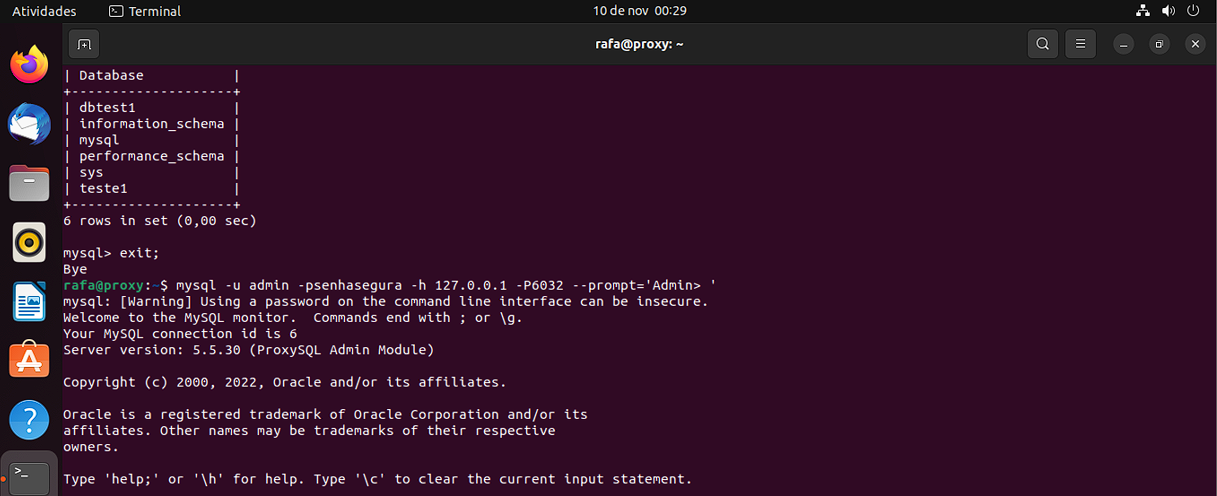
\includegraphics[width=13cm]{admin.png}
\caption{User Admin}
\end{figure}

Depois de criar o cliente, por questões de segurança, alteramos a palavra-passe original:

\begin{verbatim}UPDATE global_variables SET variable_value='admin:senhasegura' \end{verbatim}
\begin{verbatim}WHERE variable_name='admin-admin_credentials';\end{verbatim}

\newpage
A consulta acima usada foi gravada apenas em memória e para isso precisamos de copiar a configuração para o disco executando os seguintes comandos: 

\begin{verbatim}LOAD ADMIN VARIABLES TO RUNTIME;\end{verbatim}

\begin{verbatim}SAVE ADMIN VARIABLES TO DISK;\end{verbatim}

\begin{figure}[H]
\center
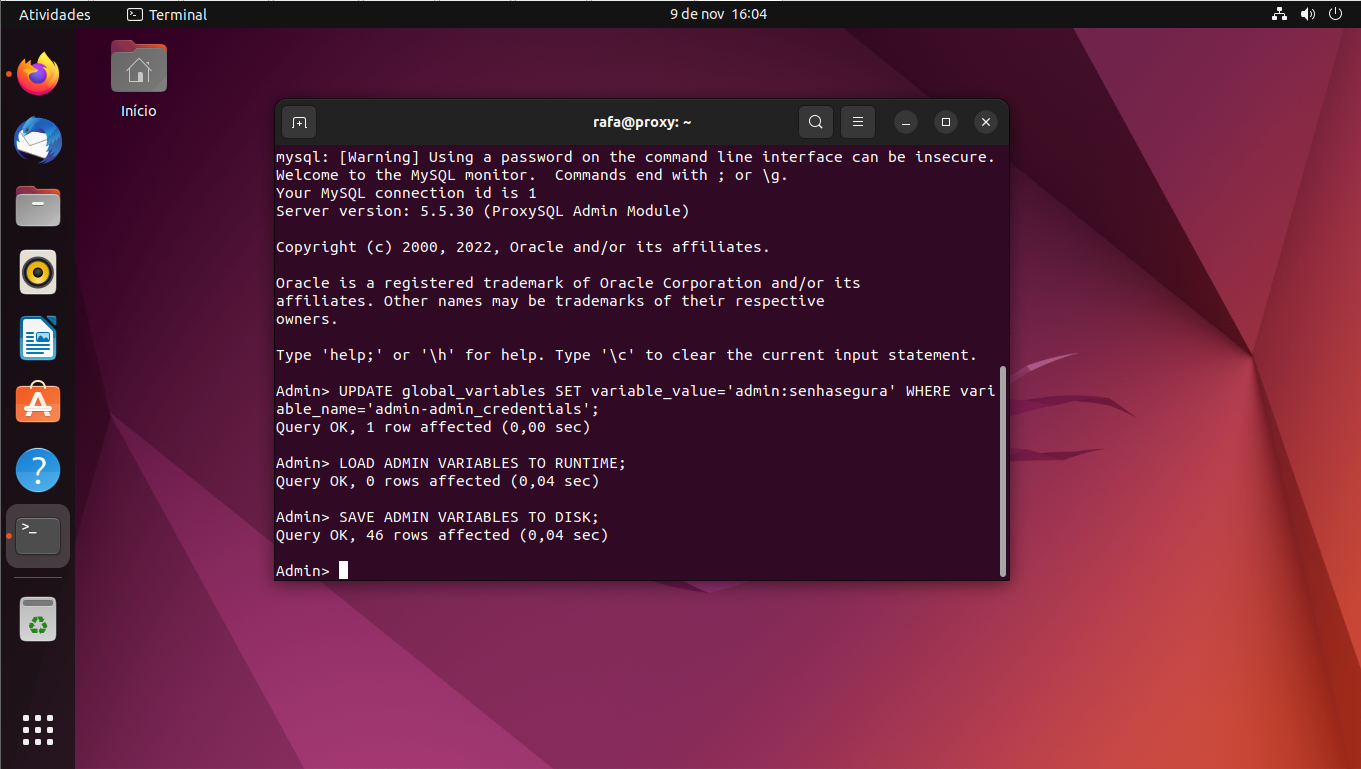
\includegraphics[width=13cm]{Screenshot_97.png}
\caption{Criação Cliente}
\end{figure}

\hfill \break
\indent A configuração ProxySQL consiste em três camadas:
\begin{itemize}
    \item Memory (memória);
    \item Disk (disco);
    \item Runtime (tempo de execução).
\end{itemize}

\newpage
\indent Passo 3: Configurar Monitorização Galera Cluster

\hfill \break
\indent O ProxySQL precisa de comunicar com os nós do cluster para conhecer o seu estado. Isto significa que o ProxySQL tem de se ligar aos nóss através de um utilizador.\\
Para isso foi criado um utilizador num dos nós e esse utilizador será replicado automaticamente através do cluster.

\hfill \break
\indent Nó 1:
\begin{verbatim}CREATE USER 'monitor'@'%' IDENTIFIED BY 'senhasegura';\end{verbatim}
\begin{verbatim}flush privileges;\end{verbatim}

\begin{figure}[H]
\center
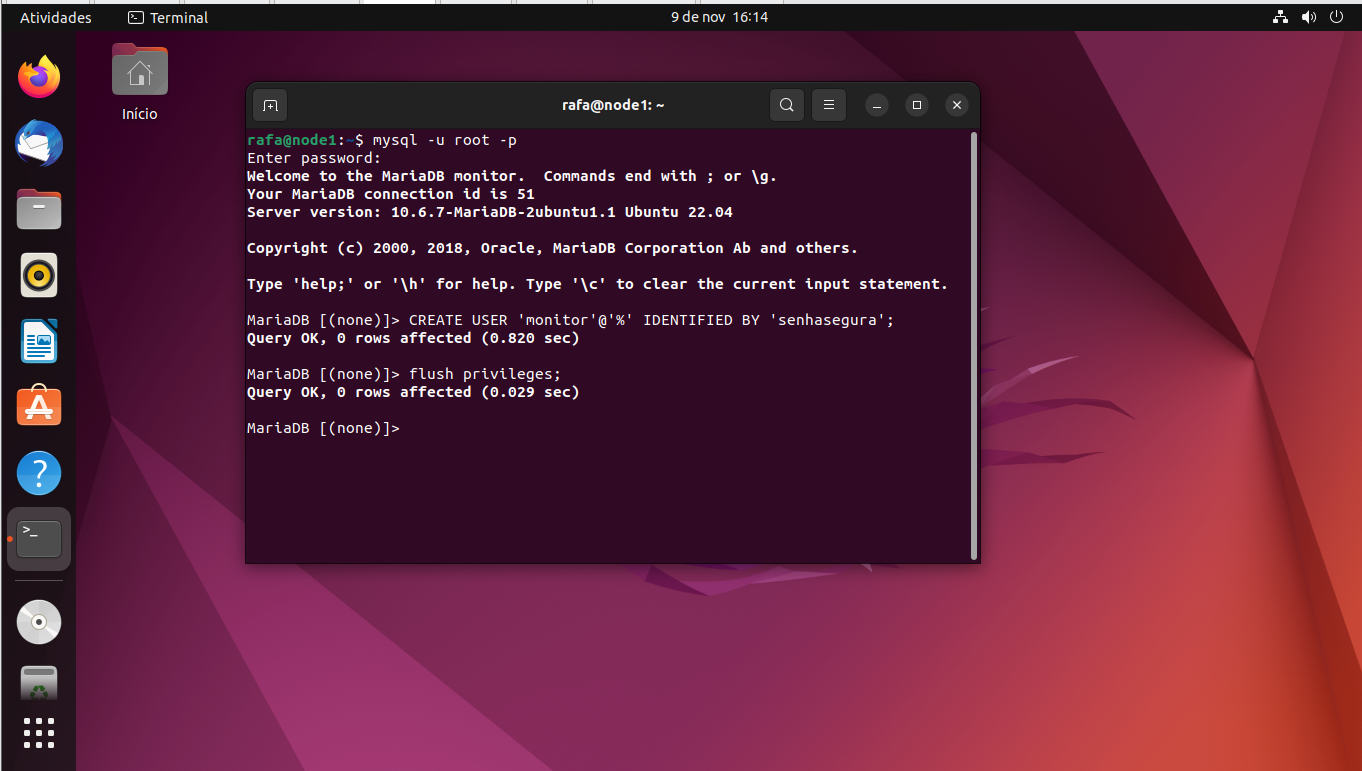
\includegraphics[width=13cm]{Screenshot_99.png}
\caption{Utilizador ProxySQL-MariaDB}
\end{figure}


\hfill \break
\indent Passo 4: Configurar Monitorização ProxySQL

\hfill \break
\indent Passamos à fase da criação do administrador do ProxySQL para monitorizar os nós.\\
NOTA: As credenciais do utilizador que configurámos no passo anterior têm de coincidir.

\begin{verbatim}
UPDATE global_variables SET variable_value='monitor' 
WHERE variable_name='mysql-monitor_username';  
\end{verbatim}

\begin{verbatim}UPDATE global_variables SET variable_value='senhasegura' 
WHERE variable_name='mysql-monitor_password';\end{verbatim}

\newpage
Definir parâmetros de intervalos na monitorização:

\begin{verbatim}UPDATE global_variables SET variable_value='2000' WHERE variable_name 
IN ('mysql-monitor_connect_interval','mysql-monitor_ping_interval',
'mysql-monitor_read_only_interval');\end{verbatim}

\begin{figure}[H]
\center
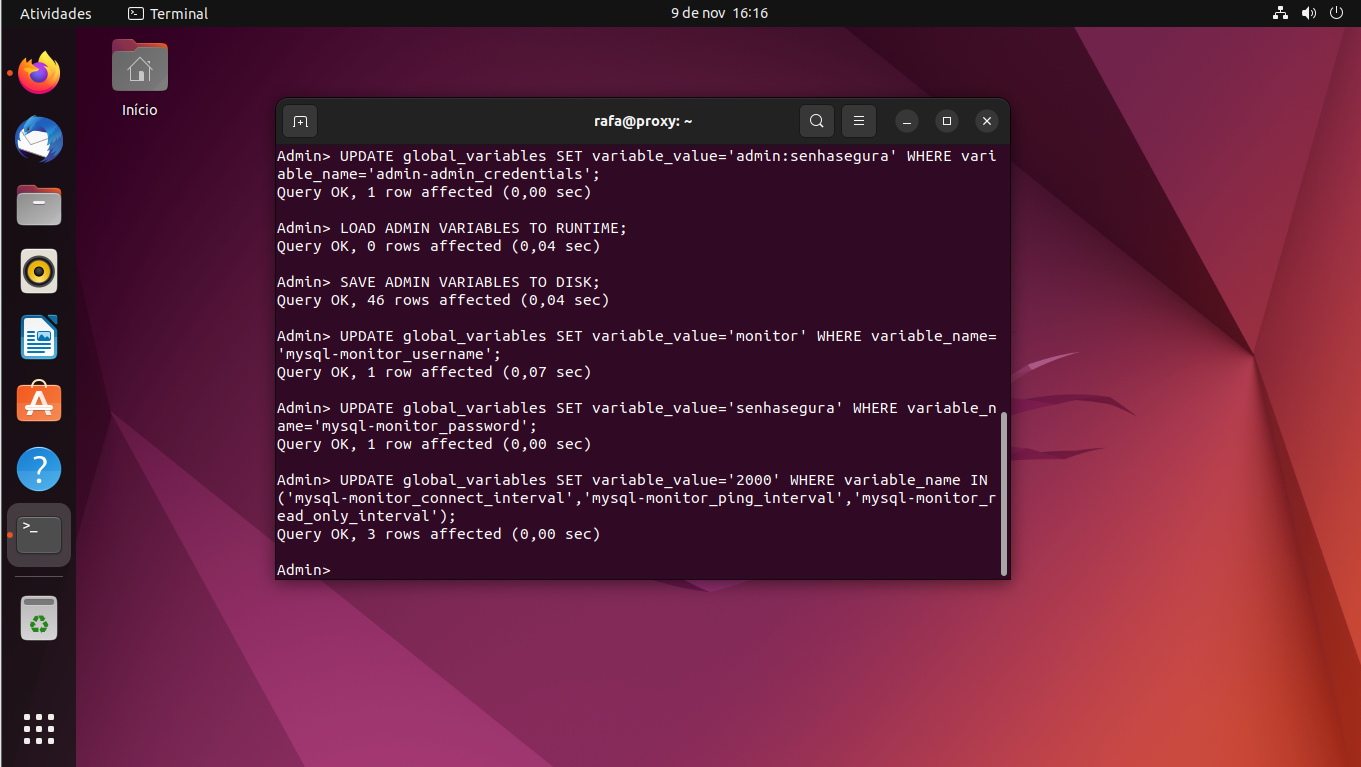
\includegraphics[width=13cm]{Screenshot_102.png}
\caption{Monitorização ProxySQL}
\end{figure}

Confirmar as alterações feitas:

\begin{verbatim}SELECT * FROM global_variables WHERE variable_name LIKE 'mysql-monitor_%';\end{verbatim}

\begin{figure}[H]
\center
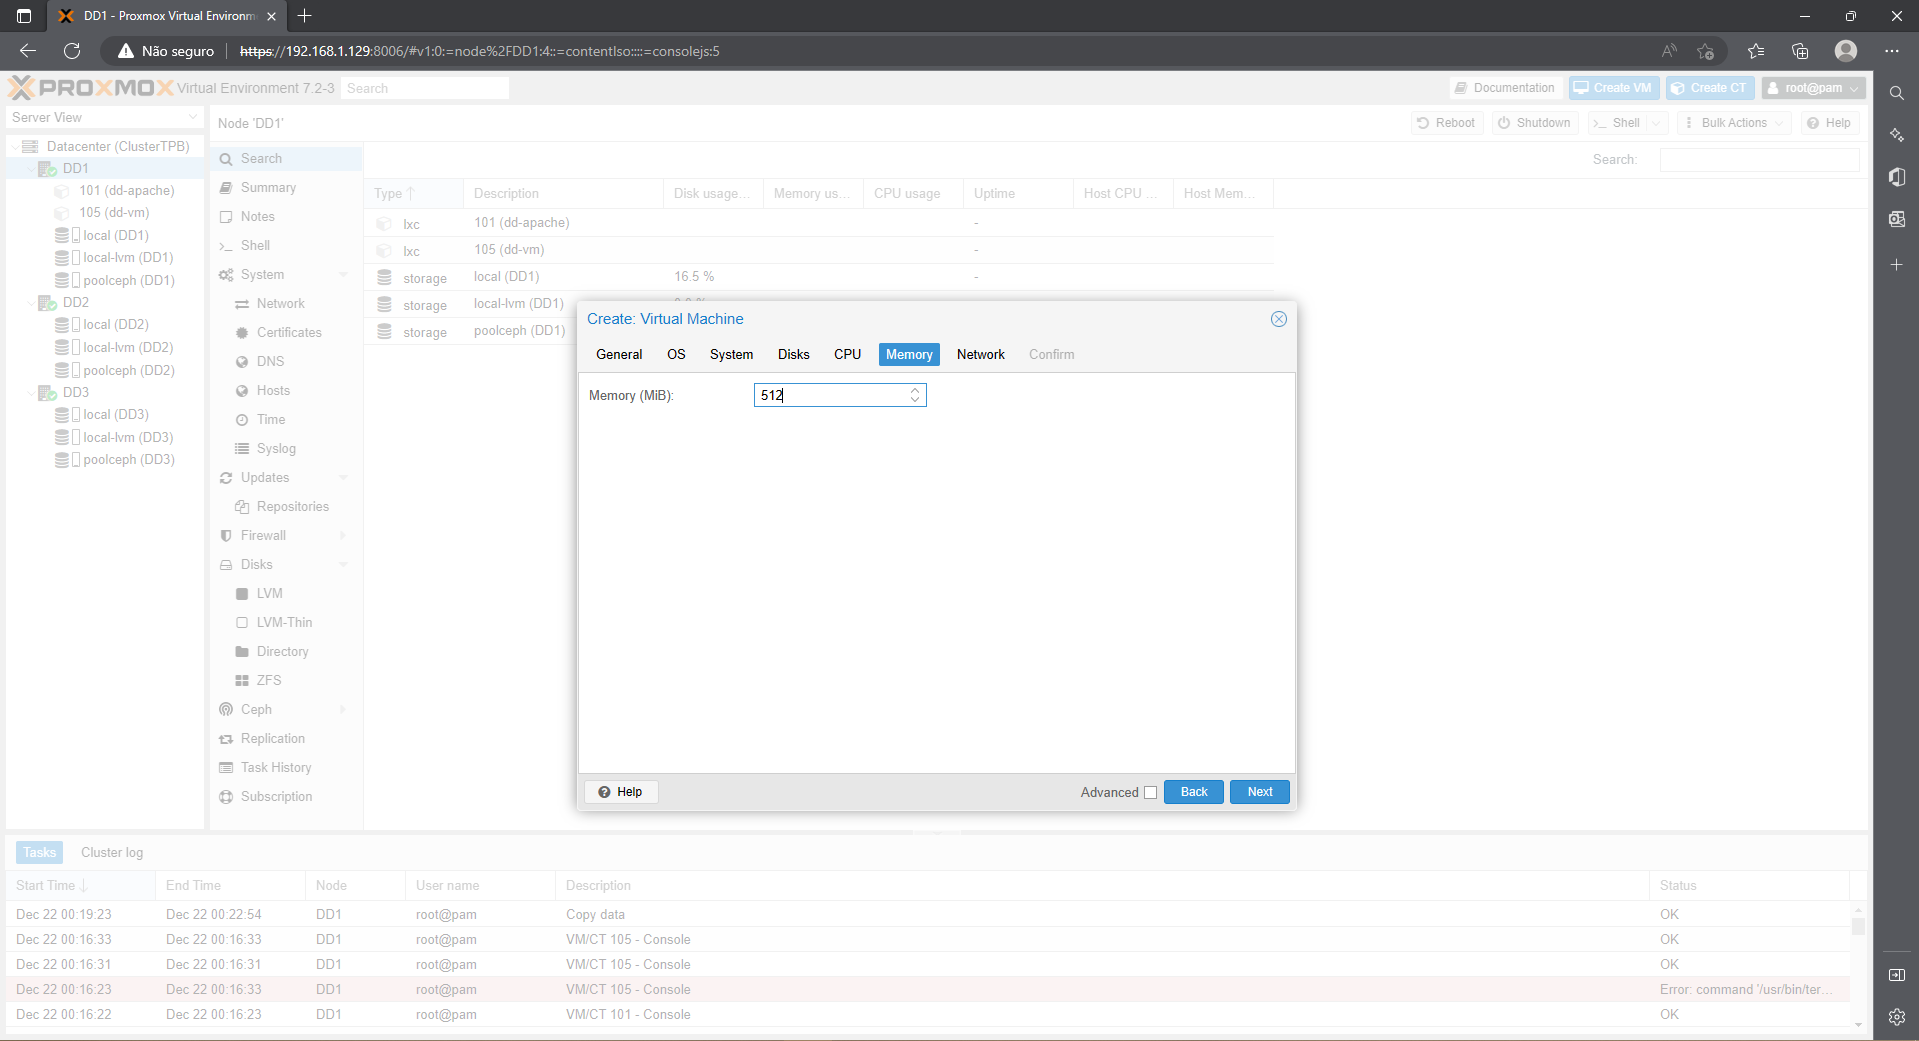
\includegraphics[width=13cm]{Screenshot_116.png}
\caption{Configurações ProxySQL}
\end{figure}

\indent Guardar as alterações realizadas:

\begin{verbatim}LOAD MYSQL VARIABLES TO RUNTIME;\end{verbatim}
\begin{verbatim}SAVE MYSQL VARIABLES TO DISK;\end{verbatim}

\newpage
Passo 5: Adicionar nós ao Backend ProxySQL\\

O passo seguinte é adicionar os três nós que existem no nosso Galera Cluster. O ProxySQL usa \textit{hostgroups} para os nós de backend. Um \textit{hostgroup} é um conjunto de nós identificados por um número positivo, 1 ou 2. O objetivo de usar \textit{hostgroups} é auxiliar as consultas do ProxySQL aos diferentes \textit{host groups}, utilizando o encaminhamento de consultas ProxySQL.

\hfill \break
\indent O ProxySQL tem os seguintes \textit{hostgroups} lógicos:
\begin{itemize}
    \item Escritores - nós que podem escrever/alterar dados (Nó Master), também são leitores. 
    \item Leitores - nós que só podem aceitar consultas de leitura (Nó Slave)
\end{itemize}

\hfill \break
\indent Próximo passo, configurar a tabela \textit{`mysql\textunderscore replication\textunderscore hostgroup`} na base de dados e especificar os \textit{hostgroups}:

\begin{verbatim}SHOW CREATE TABLE main.mysql_replication_hostgroups\G\end{verbatim}

\begin{figure}[H]
\center
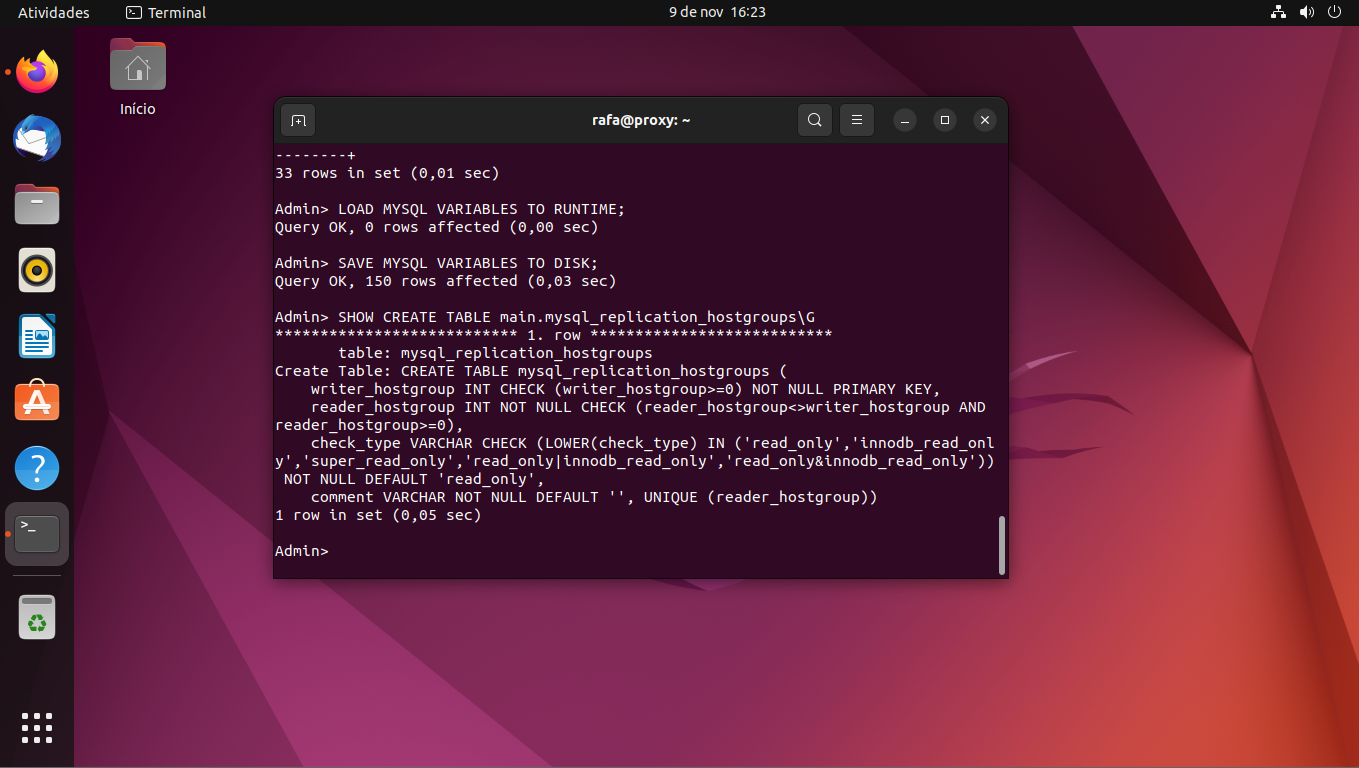
\includegraphics[width=13cm]{Screenshot_106.png}
\caption{Criação tabela mysql\textunderscore replication\textunderscore hostgroup}
\end{figure}

\hfill \break
\begin{verbatim}INSERT INTO main.mysql_replication_hostgroups (writer_hostgroup,
reader_hostgroup,comment) VALUES (1,2,'galera_cluster');\end{verbatim}

\newpage
De seguida inserir os nós no proxySQL:

\begin{verbatim}INSERT INTO main.mysql_servers(hostgroup_id,hostname,port) 
VALUES (1,'192.168.1.118',3306);\end{verbatim}

\begin{verbatim}INSERT INTO main.mysql_servers(hostgroup_id,hostname,port) 
VALUES (1,'192.168.1.119',3306);\end{verbatim}

\begin{verbatim}INSERT INTO main.mysql_servers(hostgroup_id,hostname,port) 
VALUES (1,'192.168.1.120',3306);\end{verbatim}

\hfill \break
\indent Guardar as configurações em disco:
\begin{verbatim}LOAD MYSQL VARIABLES TO RUNTIME;\end{verbatim}
\begin{verbatim}SAVE MYSQL VARIABLES TO DISK;\end{verbatim}

\begin{figure}[H]
\center
\includegraphics[width=13cm]{Screenshot_110.png}
\caption{Inserir nós ProxySQL}
\end{figure}

\hfill \break
\indent Carregar as configurações para o \textit{runtime}:

\begin{verbatim}LOAD MYSQL SERVERS TO RUNTIME;\end{verbatim}

\newpage
Confirmação de que os servidores se conectaram corretamente (conexão e ping):

\begin{verbatim}SELECT * FROM monitor.mysql_server_connect_log ORDER BY time_start_us 
DESC LIMIT 3;\end{verbatim}

\begin{verbatim}SELECT * FROM monitor.mysql_server_ping_log ORDER BY time_start_us 
DESC LIMIT 3;\end{verbatim}


\begin{figure}[H]
\center
\includegraphics[width=13cm]{Screenshot_130.png}
\caption{Conexão entre Proxy e Nodes}
\end{figure}

\indent Por fim, ainda pude verificar no Proxy o estado dos nós do cluster.

\begin{verbatim}SELECT hostgroup,srv_host,status FROM stats.stats_mysql_connection_pool; \end{verbatim}

\begin{figure}[H]
\center
\includegraphics[width=13cm]{Screenshot_131.png}
\caption{Conexão entre Proxy e nós}
\end{figure}

\newpage
Passo 6: Criação de utilizador MySQL

\hfill \break
\indent Neste passo vamos criar um utilizador MySQL que se irá ligar ao cluster através do ProxySQL. Para isso num dos nós é criado o utilziador que será replicado pelos restantes.

\begin{verbatim}create user 'rafa1'@'%' identified by 'senhasegura'; \end{verbatim}

\hfill \break
\indent Garantir que o utilizador tem privilégios para aceder a várias funções:

\begin{verbatim}grant all privileges on testdb.* to 'rafa1'@'%' with grant option;\end{verbatim}

\begin{verbatim}flush privileges;\end{verbatim}

\hfill \break
\indent Passo 7: Adicionar o utilizador MySQL ao ProxySQL

\hfill \break
\indent O registo deste utilizador é acrescentado na tabela \textit{mysql\textunderscore users} da base de dados do ProxySQL:

\begin{verbatim}SHOW CREATE TABLE mysql_users\G\end{verbatim}

Depois de criar a tabela, é inserido numa query o nome de utilizador, palavra-passe e \textit{hostgroup}:

\begin{verbatim}INSERT INTO mysql_users(username,password,default_hostgroup) 
VALUES ('rafa1','senhasegura',1);\end{verbatim}

Para terminar, falta guardar as alterações:

\begin{verbatim}LOAD MYSQL USERS TO RUNTIME;\end{verbatim}

\begin{verbatim}SAVE MYSQL USERS TO DISK;\end{verbatim}

Para confirmar, podemos verificar se o utilizador foi adicionado:

\begin{verbatim}SELECT * FROM mysql_users;\end{verbatim}

\newpage
Passo 8: Conexão do utilizador MySQL criado no passo anterior no ProxySQL.

\hfill \break
\indent Assim, podemos fazer query ás base de dados, testando a ligação e permissões criadas para o acesso ao cluster pelo ProxySQL.

\begin{verbatim}mysql -urafa1 -h 127.0.0.1 -P6033 -p\end{verbatim}

Depois de fazer login no ProxySQL com o utilizador MySQL podemos ver, por exemplo, as bases de dados existentes no cluster:

\begin{verbatim}show databases;\end{verbatim}

\begin{figure}[H]
\center
\includegraphics[width=13cm]{Screenshot_137.png}
\caption{Veirifcação Base de dados no Proxy}
\end{figure}

\newpage
\section{Instalação Wireshark}

\begin{verbatim}sudo add-apt-repository ppa:wireshark-dev/stable\end{verbatim}

\begin{verbatim}sudo apt update\end{verbatim}

\begin{verbatim}sudo apt install wireshark\end{verbatim}

Durante a instalação vamos ser notificados com uma configuração onde se pretende que seja escolhido a opção SIM ou NÃO, para utilizadores do \ac{SO} sem permissões poderem capturar pacotes, eu optei por escolher SIM. 

\begin{figure}[H]
\center
\includegraphics[width=13cm]{wire.png}
\caption{Configuring Wireshark-common}
\end{figure}

\begin{verbatim}sudo usermod -aG wireshark $(whoami)\end{verbatim}

Em algumas experiências anteriores ao abrir o Wireshark pelo atalho gerado, existia um \textit{bug} onde não aparecia na tela inicial do Wireshark as várias interfaces de rede do "computador" e para evitar esse \textit{bug} eu inicie a partir daí o Wireshark pelo terminal usando:

\begin{verbatim}sudo wireshark\end{verbatim}

Depois de aberto o Wireshark na tela inicial escolhe-se a interface de rede, no meu caso é a ens33, e começa a captura de pacotes.

\begin{figure}[H]
\center
\includegraphics[width=13cm]{Screenshot_132.png}
\caption{Wireshark}
\end{figure}

\newpage
\section{Experiência} 
Para esta experiência simulei a falha de um nó do cluster. Apenas desliguei a interface de rede na \ac{VM} 3 (nó 3), ou podia também desligar o serviço mariaDB com o comando \textit{sudo systemctl stop mariadb}.

Depois de desligar a interface de rede no nó 3 seria de esperar que este nó saísse do cluster:

\begin{figure}[H]
\center
\includegraphics[width=13cm]{Screenshot_145.png}
\caption{Tamanho do cluster depois da falha}
\end{figure}

Como podemos ver, eu tinha verificado antes de desligar a interface de rede do nó 3 o tamanho do cluster e depois do nó três ficar inativo o tamanho do cluster passou para dois, como esperado.\\
Passando para a \ac{VM} do ProxySQL fui verificar a pool dos \textit{hostgroup} e verifiquei que o nó três ficou \textit{SHUNNED}:

\begin{verbatim}SELECT hostgroup,srv_host,status FROM stats.stats_mysql_connection_pool;\end{verbatim}

\begin{figure}[H]
\center
\includegraphics[width=13cm]{Screenshot_146.png}
\caption{Pool Hostgroups}
\end{figure}

Ativei novamente a interface de rede da \ac{VM} do nó três e o cluster voltou a ficar com o tamanho de três e o nó três da pool do ProxySQL voltou ao estado inicial.

\begin{figure}[H]
\center
\includegraphics[width=13cm]{Screenshot_147.png}
\caption{Pool Hostgroups}
\end{figure}

\newpage
\section{Sysbench}
Para dar inicio ao tema do Sysbench comecei por adicionar uma nova \ac{VM} e o seu \ac{IP} como está descrito na tabela de encaminhamento no inicio do capitulo é 192.168.1.121. De seguida registo detalhadamente toda a configuração e os testes efetuados.

\hfill \break
\indent Passo 1: Instalação Sysbench

\begin{verbatim}curl -s https://packagecloud.io/install/repositories/akopytov/sysbench
/script.deb.sh | sudo bash\end{verbatim}

\begin{verbatim}sudo apt-get install sysbench\end{verbatim}

\hfill \break
\indent Passo 2: Criação Base de Dados no Cluster

\hfill \break
\indent Para este passo evitava de ter criado uma nova base de dados uma vez que já existia no cluster uma denominada "dbtest1". Então, no nó 1 comecei por criar a base de dados que serviu de teste. Como a replicação está ativa, como já expliquei anteriormente, ao criar num nó a base de dados, essa será replicada por todo o cluster.

\begin{verbatim}create database sbtest1\end{verbatim}

\hfill \break
\indent Passo 3: Diretoria 

\hfill \break
\indent A execução do teste foi feita na diretoria:
\begin{verbatim}/usr/share/sysbench/\end{verbatim}

\hfill \break
\indent Passo 4: Execução do teste

\hfill \break
\indent Para a execução do teste existem duas fases, uma onde será indicado a fase de \textit{prepare} e a segunda que será o \textit{run}.
Para o comando \textit{prepare} e \textit{run} utilizei o utilizador rafa1 com a respetiva password, o host do proxy, e a base de dados sbtest1.

\begin{verbatim}sysbench oltp_read_write --db-driver=mysql 
--table-size=100 --mysql-user=rafa1 --mysql-password=senhasegura 
--mysql-port=6033 --mysql-host=192.168.1.122 --mysql-db=sbtest1 --threads=4 
prepare --debug\end{verbatim}

\newpage
\begin{verbatim}sysbench oltp_read_write --db-driver=mysql 
--table-size=100 --mysql-user=rafa1 --mysql-password=senhasegura 
--mysql-port=6033 --mysql-host=192.168.1.122 --mysql-db=sbtest1 --threads=4 
run --debug\end{verbatim}

\begin{figure}[H]
\center
\includegraphics[width=13cm]{Screenshot_149.png}
\caption{Run Teste Sysbench}
\end{figure}

\begin{figure}[H]
\center
\includegraphics[width=13cm]{Screenshot_150.png}
\caption{Run Teste Sysbench}
\end{figure}

\newpage
Na máquina do proxy no Wireshark ainda fiz uma pequena captura de pacotes para poder verificar os \textit{SELECT} e \textit{INSERT} que o teste fez. 

Podemos verificar todos as capturas do \textit{SELECT} durante o teste, usando o comando no Wireshark \textit{mysql.query contains "SELECT"}:

\begin{figure}[H]
\center
\includegraphics[width=13cm]{Screenshot_151.png}
\caption{Query Select}
\end{figure}

Analisando um pacote verifiquei o Statement do MySQL e o seu conteúdo. Neste pacote a máquina de destino foi o 192.168.1.118 (Nó 1):

\begin{figure}[H]
\center
\includegraphics[width=13cm]{Screenshot_152.png}
\caption{Statement SELECT MySQL}
\end{figure}

\newpage
Por fim ainda verifiquei as capturas do \textit{INSERT} durante o teste, usando o comando no Wireshark \textit{mysql.query contains "INSERT"}:

\begin{figure}[H]
\center
\includegraphics[width=13cm]{Screenshot_153.png}
\caption{Query INSERT}
\end{figure}

Analisando um dos pacotes verifiquei o Statement do MySQL e o seu conteúdo. Neste pacote a máquina de destino foi o 192.168.1.119 (Nó 2):

\begin{figure}[H]
\center
\includegraphics[width=13cm]{Screenshot_154.png}
\caption{Statement INSERT MySQL}
\end{figure}